\documentclass[11pt]{article}
\usepackage{lipsum} 
\usepackage{amsmath}
\usepackage{graphicx}
\usepackage{geometry}
\usepackage{csquotes}
\usepackage{endnotes}
\usepackage{hyperref}

\graphicspath{ {./images/} }
\geometry{
    left=2.5cm,
    right=2.5cm,
    top=3cm,
    bottom=3cm
}
\usepackage[english]{babel}

\title{Lovecraft}
\begin{document}

    \section*{Analyzing the Works of H.P. Lovecraft in Thematic Correlation to his Personal Life}
    Projektarbeit zum Modul: Einführung in Digital Humanities, Wintersemester 2022/23\\
    Repository: \href{https://github.com/Nachtschrecken/Lovecraft_TopicModel}{https://github.com/Nachtschrecken/Lovecraft\_TopicModel}\\\\
    Autor: Ferris Kleier\\
    Matrikelnummer: 3732130\\
    Studiengang: Informatik B.Sc.\\
    Datum: 05. März 2023

    \section{Introduction}

This project aims to analyze the works of Howard Phillips Lovecraft, one of the most known horror 
authors, in regard to their themes and patterns. This will be done using 
topic modeling on all of his writings to collect a timeline-like collection of the most common 
themes in his works. H.P. Lovecraft highly contributed to the modern horror genre with his 
detailed descriptions of cosmic horror (a term defined by his writings) and stories about 
monsters and scary events. While his writings are known for complexity and style, his thematic 
and contextual depth is equally impressive and the subject of this project. Therefore, Lovecraft 
is well-known by fans of horror and science fiction literature, like Stephen King, who stated 
that Lovecraft heavily influenced his style and ideas. \\

Even though Lovecraft lived from 1890-1937 and did not encounter computers or other devices of 
our current age, his works and letters are digitalized and preserved for reading and research. 
One key aspect of this project is to apply the digital humanities method of topic modeling on 
all of Lovecraft’s works. The digital humanities is a field of study, research, teaching, and 
invention concerned with the intersection of computing and the disciplines of the humanities. 
One can think of it as a bridge between the two cultures of natural science, which tries to 
explain what is going on, and humanities, which tries to understand what is happening. One key 
figure in this field is Roberto Busa (1913 - 2011), who used computational methods to create a 
collection of all the words of Thomas Aquinas, later known as the Index Thomisticus. He 
achieved his goal with the help of IBM, at that time one of the biggest computer manufacturers, 
and connected his studies with the help of digital computing to process the millions of words 
he strived to process.\\

By using the digital humanities, we can gain new insights on Lovecraft’s writings and identify 
recurring themes, patterns, and motifs in the big corpus of his writings. The methods used in 
the digital humanities include Stylometry, Topic Modeling, Network Analysis, and 
Geovisualization. For the purpose of this project, we will use topic modeling to gather 
insight into the large corpus and structure the results like a timeline for every one of 
his works. Regarding digital humanities, this project aims to explore the humanities of 
literature and apply computational methods on it. That way we can see the most occurring 
themes from his first works to his last ones and compare them in terms of lore consistency 
(how did his themes and mythos change?), social correlation (does he refer to social events 
of his time?) and comprehensive insight on the different features of his works. Some works 
already covered features of his writings and life like the fear of progress, dangers of 
scientific progress, and persistence of ancient evils.
    \section{Research Agenda}
    \section{Data Overview}

The data for this project can be found on Kaggle. We decided to go with this dataset because 
it features all of Lovecraft’s written texts in .txt. format, which makes it easy to process 
the data. All stories exist in public domain and are not subject to copyright. Due to the 
stories being public domain, and more datasets being available online as well as raw HTML 
texts available, we had many sources to choose from. A comparison with other sources and 
physical prints of stories does not indicate any biases or alteration in the texts. Though 
we have found some works in the dataset that are not solely written by Lovecraft, since he 
collaborated with many other authors of his time and even took ghostwriting commissions. 
Another problem also occured with other datasets, where the earliest works of Lovecraft 
are missing. We decided to still go with this dataset and remove works which we don’t want 
to include. Since our research question wants to only cover Lovecraft’s ideas and writings, 
the influence from other authors or commissioners could alter the results. That’s because 
the ideas of Lovecraft are not really present in these specific writings, though his 
stylometry may be the same.\\

The dataset contains 102 works of Lovecraft, including all collaborations. As we just 
mentioned, collaborations, revisions and ghost writings are not subject of this project 
and will be removed. An overview of all the works written solely by Lovecraft, his fiction, 
can be found in his bibliography on Wikipedia. In this case only his ‘fiction’ will be 
included in this project as well as some of his works found under ‘Juvenilia’, which 
include his earliest writings when he was young. Also not included in this project are 
his poetry works, philosophical works and scientific works since they are either too 
short or provide no information in regard to his mythos and lore. After only keeping 
the works of Lovecraft from the bibliography the dataset has remaining 70 stories. 
These works can be distinguished into short stories, novellas, or even fragments from 
letters or novellas. Lovecraft’s works largely vary in length, some just a few pages, 
and other whole novellas. Fragments could also contain just a few paragraphs. One example 
is the story ‘Azatoth’ (written June 1922), which is very short in length and was 
supposed to be part of a whole novella, though only this fragment survived. It is currently 
unknown how many such fragments were lost, but his wife admitted to have burned a lot of 
his letters. If these included other fragments or whole works of Lovecraft not yet 
published or copied at that time, that means there were works which are lost forever.\\

The 70 works in this modified dataset are .txt documents. The text files contain the 
title and the raw text. We formatted the files using R and pasted them into a .csv 
format. In this process we also added the dates as a second row to the text and manually 
put another line between paragraphs process them using regular expressions. The file to 
process the dataset can be found in the repository as ‘format.r’. The .csv file contains 
for every text the text\_id, then for every paragraph of the text the doc\_id, the title, 
the date, and the paragraph containing the text. This way we can later use topic modeling 
on the csv to create a timeline-like plot of the main themes. The dates found in different 
sources can be misleading, since some stories were published after Lovecraft’s death. 
One example is the story ‘The Case of Charles Dexter Ward’, which was written in 1927, 
partly published in 1941, and fully published in 1943, while Lovecraft already died in 
1937. The dates we manually added to each file represents the date a work was written 
as provided on WikiSource. This corresponds better to his personal life and events. 
For dates where only the year is provided (see ‘The Alchemist’, 1908) or no explicit 
month (see ‘The Street’, late 1919) we used proper months according to quarters or the 
beginning of seasons. For plain years we added the January of that year. Taking into 
account publishing dates is no option, since they do not reflect Lovecraft’s personal 
events, may not be in order, or even have been published after his death as already 
mentioned.\\



    \section{Method Overview}

In the digital humanities, there are four main methods to work on data and achieve information. 
Stylometry is a method to find textual similarities between texts, Network analysis can be used 
to find relations in data, Geovisualization is used to representing data on maps, and the fourth 
method, which we will use for this project, is topic modeling. Topic modeling is a method to 
gather information from texts regarding the content. Using this computational approach we can 
uncover the main themes and topics from texts, not just by using a frequentist method with the 
most words used, but by putting context in the found information. A topic model achieves this 
while it discovers the degree to which each document exhibits those topics. That way we can 
build a statistical lens that encodes our specific knowledge, theories, and assumptions about 
texts \cite{blei}.\\

Using topic modeling on the collection of Lovecraft's works will help us uncover the most 
important themes per text regarding not only the frequentist quantity of certain topics but, 
as already mentioned, the contextual frequency. We want to know what topic dominates each text, 
and topic modeling is exactly the tool we need for that. By writing short scripts in the 
programming language R, we can compute the main topics easily and even visualize them in plots. 
For example, the R package \textit{ggplot2} is an easy tool to plot the results in a timeline-style plot. \\

We will apply topic modeling to each text. This is done because if we would use chunks of text 
over the whole concatenated collection, we would lose the important context. Especially in this 
literature of fantasy and horror, we need to keep the topics regarding their text. In one text 
like 'The Thing on the Doorstep' (written 1933) the main topic may refer to \textit{creature,
darkness, house} or others. But another text like 'The Nameless City' (written 1921) may 
yield topics like \textit{place, sculpture} and \textit{ancient}. When using chunks of a concatenated 
collection of his writings, we would use the context of each text. Therefore we work on each 
text separately, even if some texts are significantly shorter than others.\\

To reflect on some biases with this approach, we have to particularly emphasize this problem: 
Some works of Lovecraft are shorter than others. Though we do not expect any major differences 
in contextual topics between short and long texts, this has to be noted. A measure we use to 
counter this is computing a topic model using paragraphs of similar size for every work. 
According to the word count of Lovecraft's works the length of his works linearly increases 
with the years of writing. Another major bias in topic modeling is the approach of Natural 
Language Processing (NLP). For our purpose, we will work with English libraries, stopwords, 
and dictionaries. This could lead to problems when it comes to topics that do not reflect the 
English language. Lovecraft is known for his monsters and cosmic words like \textit{Necronomicon} or 
\textit{Cthulhu}. For this, we will focus on topics and words that are subject to the English language 
and can be covered by NLP. We will also keep in mind that in Lovecraft's style, specific words 
tend to occur more often than others in the literary context.
    \section{Related Work}

In this chapter, we will cover some related work that represents use cases of topic modeling 
similar to our research question. They analyze either Lovecraft's works or compare topics 
between Lovecraft's works and films and other authors.\\

The first related work is the paper 'Beyond the mountain of madness: a look at the shared 
themes of Edgar Allan Poe and H.P. Lovecraft' by Kristoffer Gustafson. This paper compares 
the main themes of both H.P. Lovecraft and Edgar Allan Poe, another well-known author, and 
poet. Poe heavily influenced Lovecraft's fiction and literary style, as he stated in his essay 
'Supernatural Horror in Literature'. The author examines the themes of insanity, death, and the 
gothic setting on both authors and projects similarities that suggest an influence of Poe on 
Lovecraft.\\

Another paper is 'The Lovecraft Look: An Examination of Lovecraftian Themes in Film' by 
Michael A. Church. The author analyzes the philosophical beliefs and life experiences that 
inspired Lovecraft's 'weird fiction' and his literary philosophy of 'Cosmic Indifferentism' 
and compares them with films influenced by Lovecraft. Lovecraft's philosophy has been heavily 
misconstrued, as evidenced by several films that purport to adapt his stories, but actually 
ignore or misinterpret Cosmic Indifferentism. However, some films successfully adhere to 
Lovecraft's focus on cosmic horror and humanity's insignificance, even if they are not direct 
adaptations of his work. The relevant task of uncovering topics gets applied in this project 
to compare Lovecraft's works and these films.\\

The third related work, 'Re-visioning Romantic-Era Gothicism: An Introduction to Key Works 
and Themes in the Study of H.P. Lovecraft' by Philip Smith, is similar to our research 
question. The author examines the recurring themes of language, genre, literary influences, 
xenophobia, cosmic indifferentism, dreams, time, and the influence of Lovecraft. Contrary 
to our work, this paper focuses on the criticism of Lovecraft. As we said in our research 
agenda, Lovecraft was known for racist slurs and regarding our modern society, these have 
to be reflected. The paper does not cover all of Lovecraft's work and the key topics to be 
uncovered correlate to major critical responses.
    \section{Experiment Design}

We apply the computational approach of topic modeling by using the R programming language and 
orient on an approach provided by A. Niekler. The R scripts as well as the optimized dataset, 
stopwords and a simple dictionary can all be found in our repository on GitHub. The file 
dict.txt contains a baseform of english vocabulary with stemmed word forms used to stem words 
and get their original lemmatization. For the processing of data we also remove stopwords 
(found in stopwords.txt) since they tend to occur as noise in the retrieved topics. 
Furthermore, we will remove some words in the preprocessing step that occur often in Lovecraft 
works but do not really represent specific related motifs for each text. For this project 
we defined the terms and names to drop because of frequency in top\_words.txt after reviewing 
the word count and first iterations of the model. We dropped names as well since they tend 
to occur more frequent than other words and did not yield any more information in the first 
iterations. On name we did keep for this experiment is ‘Carter’. That’s because Lovecraft 
maybe used the character Randolph Carter as his alter ego in the stories, since they shared 
many personal traits.\\

After preprocessing the data, we will calculate the topic model. For the topic model 
calculation we will use a Latent Dirichlet Allocation model using the R package topicmodels. 
LDA (Latent Dirichlet Allocation) is a statistical model used for topic modeling in natural 
language processing. This model assumes that documents are generated from a mixture of topics, 
and each topic is represented as a distribution over words. In the calculation process we get 
the topic model by only considering terms with a certain minimum frequency in the body of F=3. 
This is to reduce the overhead of topic that will certainly not be valuable at all and can 
already be dropped in this step. The next step includes the already mentioned drop of domain 
specific words. For LDA models, the number of topics is the most important parameter to 
define. If K is too small, the collection is divided into a few very general semantic contexts. 
If K is too large, the collection is divided into too many topics of which some may overlap 
and others are hardly interpretable. After consulting on ‘Determining the Number of Topics 
to Retain using Tools from Factor Analysis’ by Homles Finch, we decided to choose K=15 topics 
for our purpose. To facilitate a qualitative control between the retrieved topics and original 
texts, we will work with two corpus objects in this step. One being the preprocessed corpus 
to calculate the topic model overall and another original corpus. For the parameters of R 
packages like topicmodels used in the R script files, we varied them during the experiment 
process several times and sticked with the final version in our repository since they reflect 
the best use for our research question. The parameters are: a minimum of 6 counts per token 
in the corpus, 100,000 iterations, 5 terms per topic, verbose of 10, and alpha of 0.2. Other 
parameter options did not satisfy our purpose, were too short to give enough detail or too 
long to compute without further advancements.\\

After calculating the topic model, the details get visualized as results in different forms 
like a plot representing a timeline using the ggplot package in R or using the LDAvis package 
in R to gain more information on topics. LDAvis calculates the importance of a topic by 
determining how much probability is assigned to the topics. We can also filter the topics 
in our advance, e.g. to filter for specific names of monsters or places from the Cthulhu 
Mythos. With these results we can then pick the main themes of Lovecraft’s works and compare 
them according to time and event in his personal life in the chapter ‘Results and Discussion’.\\

    \section{Results and Discussion}

For the results of this Project, we represented the retrieved topic model in plots. For one we 
used a simple plot package, ggplot in R, to represent every of Lovecraft’s works in chronological 
order with their distribution of the topics. We also used the R package LDAvis to show correlations 
between the topics and use an interactive interface to see the importance of relevant terms with 
respect to a topic. The resulting topics are as follows:

\begin{enumerate}
    \itemsep0em
    \item thing, time, feel, mind, life
    \item thing, horror, eye, black, sound
    \item dream, city, day, night, strange
    \item room, door, hand, floor, window
    \item place, wall, stone, vast, foot
    \item west, specimen, work, lake, body
    \item letter, curwen, time, late, charles
    \item street, house, hill, place, town
    \item family, child, son, home, time
    \item thing, folk, time, good, obed
    \item voice, sound, begin, word, time
    \item tomb, night, fear, thing, remain
    \item land, city, sea, dream, water
    \item thing, night, place, talk, people
    \item carter, ghoul, cat, night-gaunts, ship
\end{enumerate}

\begin{figure}[ht]
    \centering
    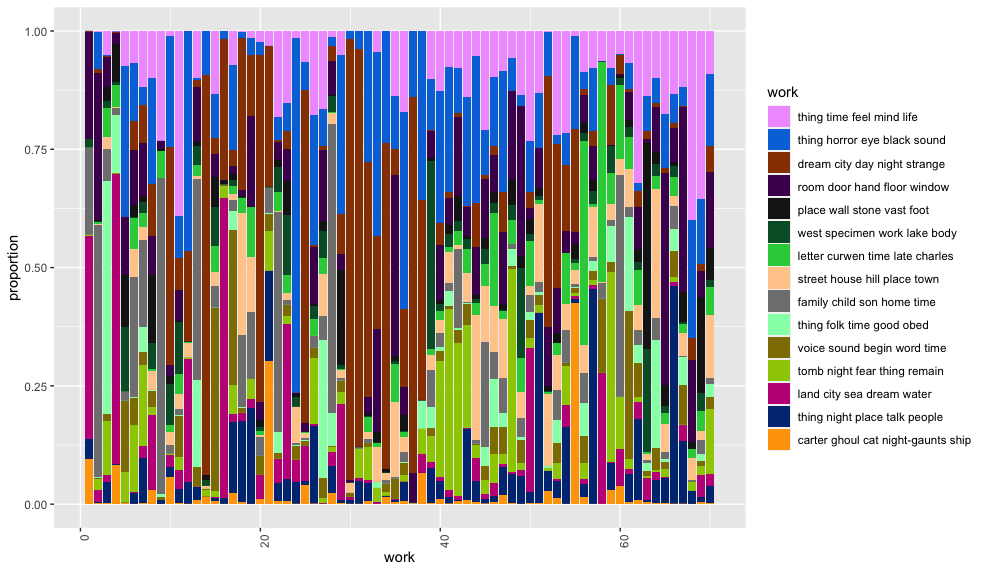
\includegraphics[width=1\textwidth]{/Users/ferriskleier/PECK/DigitalHumanities/Lovecraft_TopicModel/Project/images/plot.png}
    \caption{The plot assigning the proportion of a topic to each story of Lovecraft}
    \label{fig:mesh1}
\end{figure}

Figure 1 shows the bar chart we created to plot every of Lovecraft’s stories in chronological order 
with the percentage of the topic they share. On the x-axis, you can see the number of the story. 
Keep in mind that we used the date Lovecraft wrote the story and changed unspecified dates like just 
a year to the January of that year. For the enumeration of his works to compare to this figure, see 
stories\_list.txt. On the y-axis, you can see the distribution in percentage. Each bar corresponds to 
one work and the percentage of a topic across each of the topics in that work. The order for each 
topic per entry is the same, it’s not ordered by percentage but by topic. On the right-hand side, you 
can find the colors for each topic, pink being topic 01 consisting of the words ‘thing, time, feel, 
mind, life’.\\

The bar chart clearly shows that some topics dominate a story and others have a fairly distributed 
amount of topics. For example, the first topic in pink is highly present in some works. For 
work 55, ‘The Dream Quest of Unknown Kadath’ (written 1927) one can see that topic 15 is highly 
present, which satisfies the expectation because it is a fairly long work with a unique setting 
and motif. Another example is work 63, ‘At the Mountains of Madness’ (written 1931), the topics 
5 and 6 are more present than in any other work, which again satisfies the expectation for this 
work being unique in the antarctic setting and length. The bar chart also shows batches of topics 
for several time frames, like his works 30 to 38 which are dominated by topic 3. After reviewing 
the topic distribution for every work, we were very satisfied with the results and decided to use 
this resulting topic model for further examination.\\

To put this into context with Lovecraft’s personal life, we took several events that may have had 
a significant influence on him and checked for the topics of that time. We reviewed ‘An Epicure in 
the Terrible’ (Edited by David E. Schultz and S.T. Joshi) which is a perfect collection of essays 
by different authors regarding Lovecraft’s life. Topic 2 being blue clearly shows the time Lovecraft 
began to write the ‘Dream Cycle’, since the topics correlate well with the stories. For work 10, 
‘Polaris’ (written 1918), and work 14, ‘The White Ship’ (written 1919), one can see the high share 
of topic 3, which just continues for later stories in the dream cycle as well. This is due to the 
fact that around this time, Lovecraft met Lord Dunsany, who Lovecraft admired and who heavily 
influenced his early works which led to the dream cycle. For the works 24 (‘Nyarlathotep’, 
written 1920), 26 (‘From Beyond’, written 1920), and 29 (‘The Nameless City’, written 1921) 
topic 2 is highly present and these works mark the first shift in Lovecraft’s writings towards 
cosmic horror, which later caused the works of the ‘Cthulhu Mythos’. Starting from work 30, ‘The 
Quest of Iranon’ (written 1921), topic 3 dominates parts of his writings. Topic 3 is a good indicator 
for writings covering the dream cycle, which matches the works. The first interesting correlation 
between Lovecraft’s personal life and the graph can be seen starting from work 33, ‘The Outsider’ 
(written 1921), with topic 2 (blue) having a great share for some works and before. This may relate 
to the death of his mother in May 1921. Not only did he not write for a short period, but topic 2 
consists of the keywords ‘thing, horror, eye, black, sound’ which suggests a coping to his mother’s 
death as well as the time before may having an impact on this topic as well because she was admitted 
to a hospital. Lovecraft moved to Brooklyn in 1922 and married his wife, Sonia Haft Greene, which 
can be seen in a clear shift in topics during the time around work 39 and following, putting a break 
on the dream cycle and prompting topic 12 to be more present. Topic 12 ends being more present starting 
from work 44, ‘The Festival’ (written October 1923). That’s interesting because he did also write just 
one story for almost two years during that time, which goes in hand with his marriage and time in New 
York. Lovecraft started writing again when in 1925 he moved to Red Hook, Brooklyn, living alone 
because his wife worked somewhere else. It is known that Lovecraft despised Red Hook and was 
negatively standing against minorities that lived there. The only observable difference is, that 
topics 4, 5, and 9 started to have a stable share starting from that time. This started with his 
first story after the break ‘The Horror at Red Hook’ (written 1925) which strongly suggests his 
cope with living there. The next observable pattern begins with work 52, ‘The Strange High House 
in the Mist’ (written 1926), which is represented with a higher amount of topic 3 being the topic 
that indicates the continuation of the dream cycle. This is very interesting, because Lovecraft 
moved back to Providence in April 1926, resulting from his growing homesickness and that he became 
increasingly depressed by his isolation and the masses of “foreigners” in the city. The observation 
of topic 3 being more present again due to the continuing dream cycle indicates this. Another 
interesting correlation with Lovecraft’s stay in Brooklyn comes from topic 13. This topic covers 
terms like ‘sea’ and ‘water’ that are somewhat lacking during his time away from Providence (1922 
to 1926, work 37 to 49). This comes from the fact that Lovecraft was inspired by Providence and 
the nearby sea, though Brooklyn was close to the sea too, it was the city that influenced Lovecraft’s 
themes at that time. For ‘The Dream Quest of Unknown Kadath’ (work 55), it’s probably the most 
important work of the dream cycle and covers the fictional character Randolph Carter, who was 
supposedly an alter ego of Lovecraft as mentioned earlier. The graph also suggests a lower share 
of the first topic during the timeframe for the works covered by that topic, work 56-61 from spring 
1927 to 1930. This correlates to the fact that he divorced in 1929 and there may have been first 
signs of a shift in themes and motifs caused by unknown problems in his and Greene’s relationship 
prior to the divorce. Topic 2 is present in some of the last works again as well as topic 1 having 
a higher share starting at work 62, ‘The Thing on the Doorstep’, which was written in the summer of 
1930. This and the higher share of topic 4 starting from work 65 (‘Dreams in the Witch House’, written 
1932) indicate an observable shift in topics following a break from writing because of the death of 
his aunt Mrs. Clark in 1932 and moving with his other aunt Mrs. Gamwell into small quarters in 
Providence. He was very close with aunt Mrs. Clark and her death could be represented in the shift 
starting at work 65 where topics 4 and 14 become highly present and topic 1 having a noticeably 
higher share from work 68. Another explanation for this mix of topics during the last years could 
be that Lovecraft had a hard time selling his longer stories and concentrated on ghostwriting and 
non-fiction, resulting in the fictional works he wrote being less frequent but longer and more 
focussed on different topics.\\

\begin{figure}[ht]
    \centering
    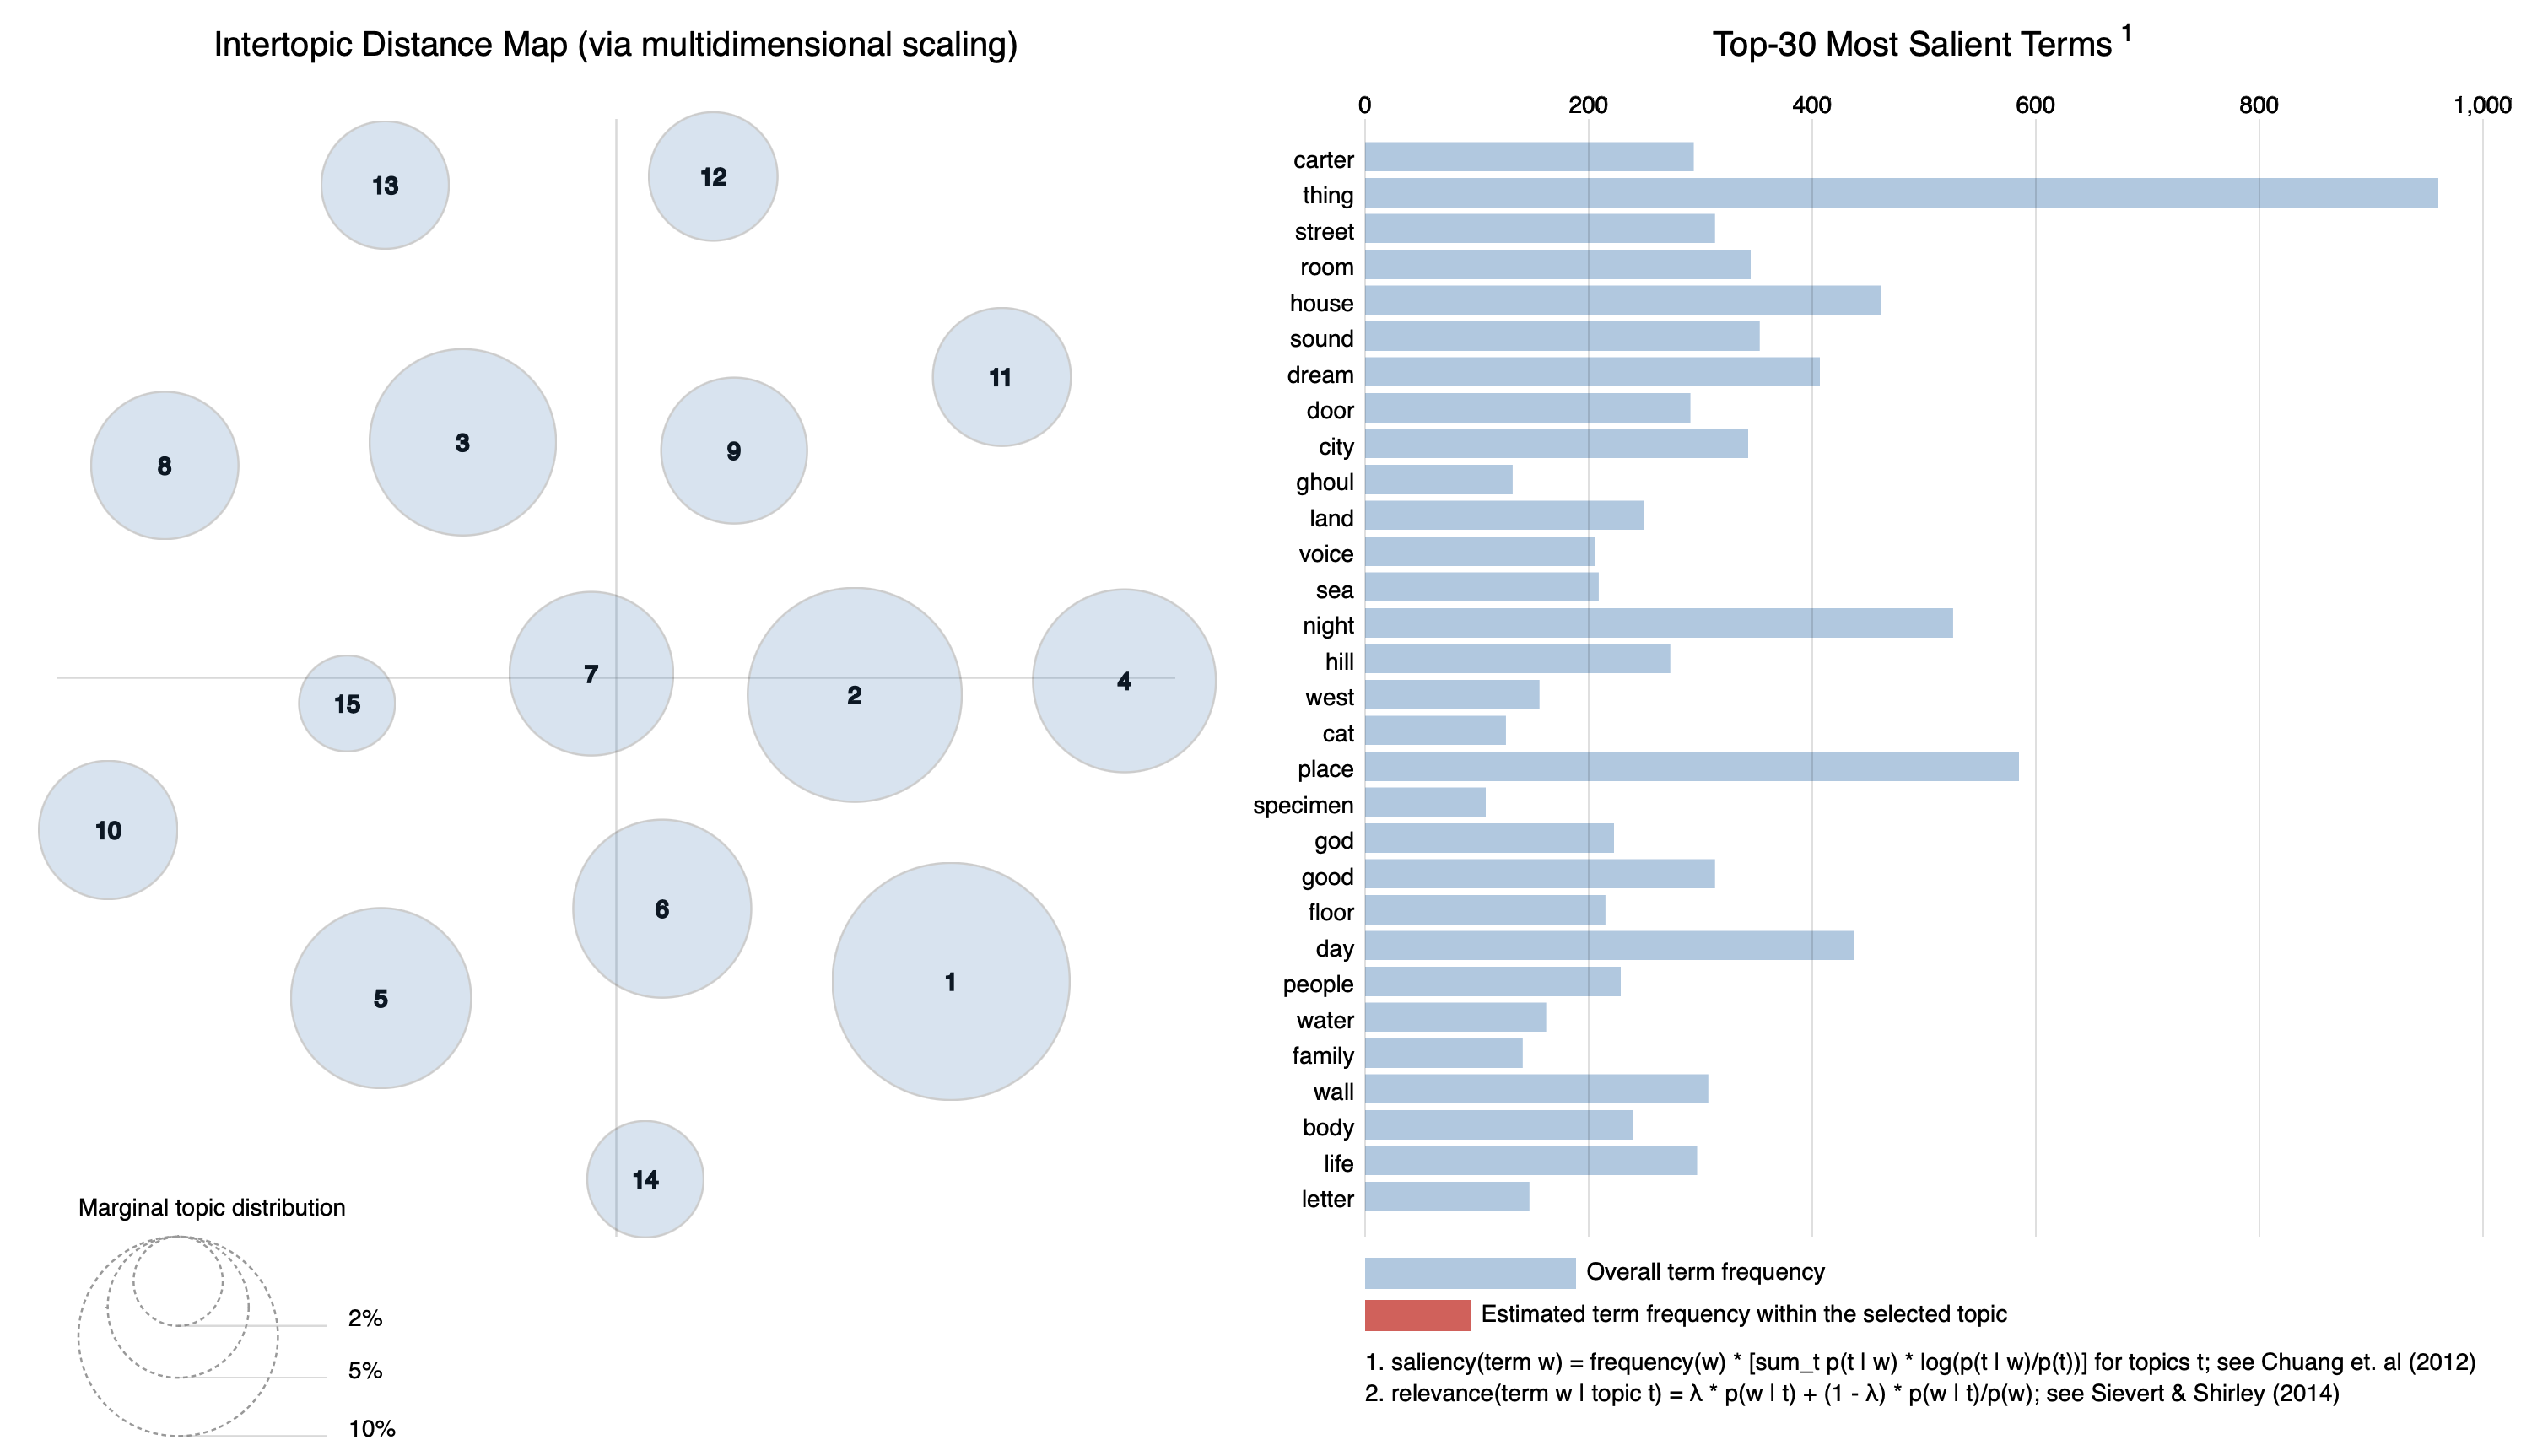
\includegraphics[width=1\textwidth]{/Users/ferriskleier/PECK/DigitalHumanities/Lovecraft_TopicModel/Project/images/ldavis_model.png}
    \caption{LDAvis results}
    \label{fig:mesh2}
\end{figure}

\begin{figure}[p]
    \centering
    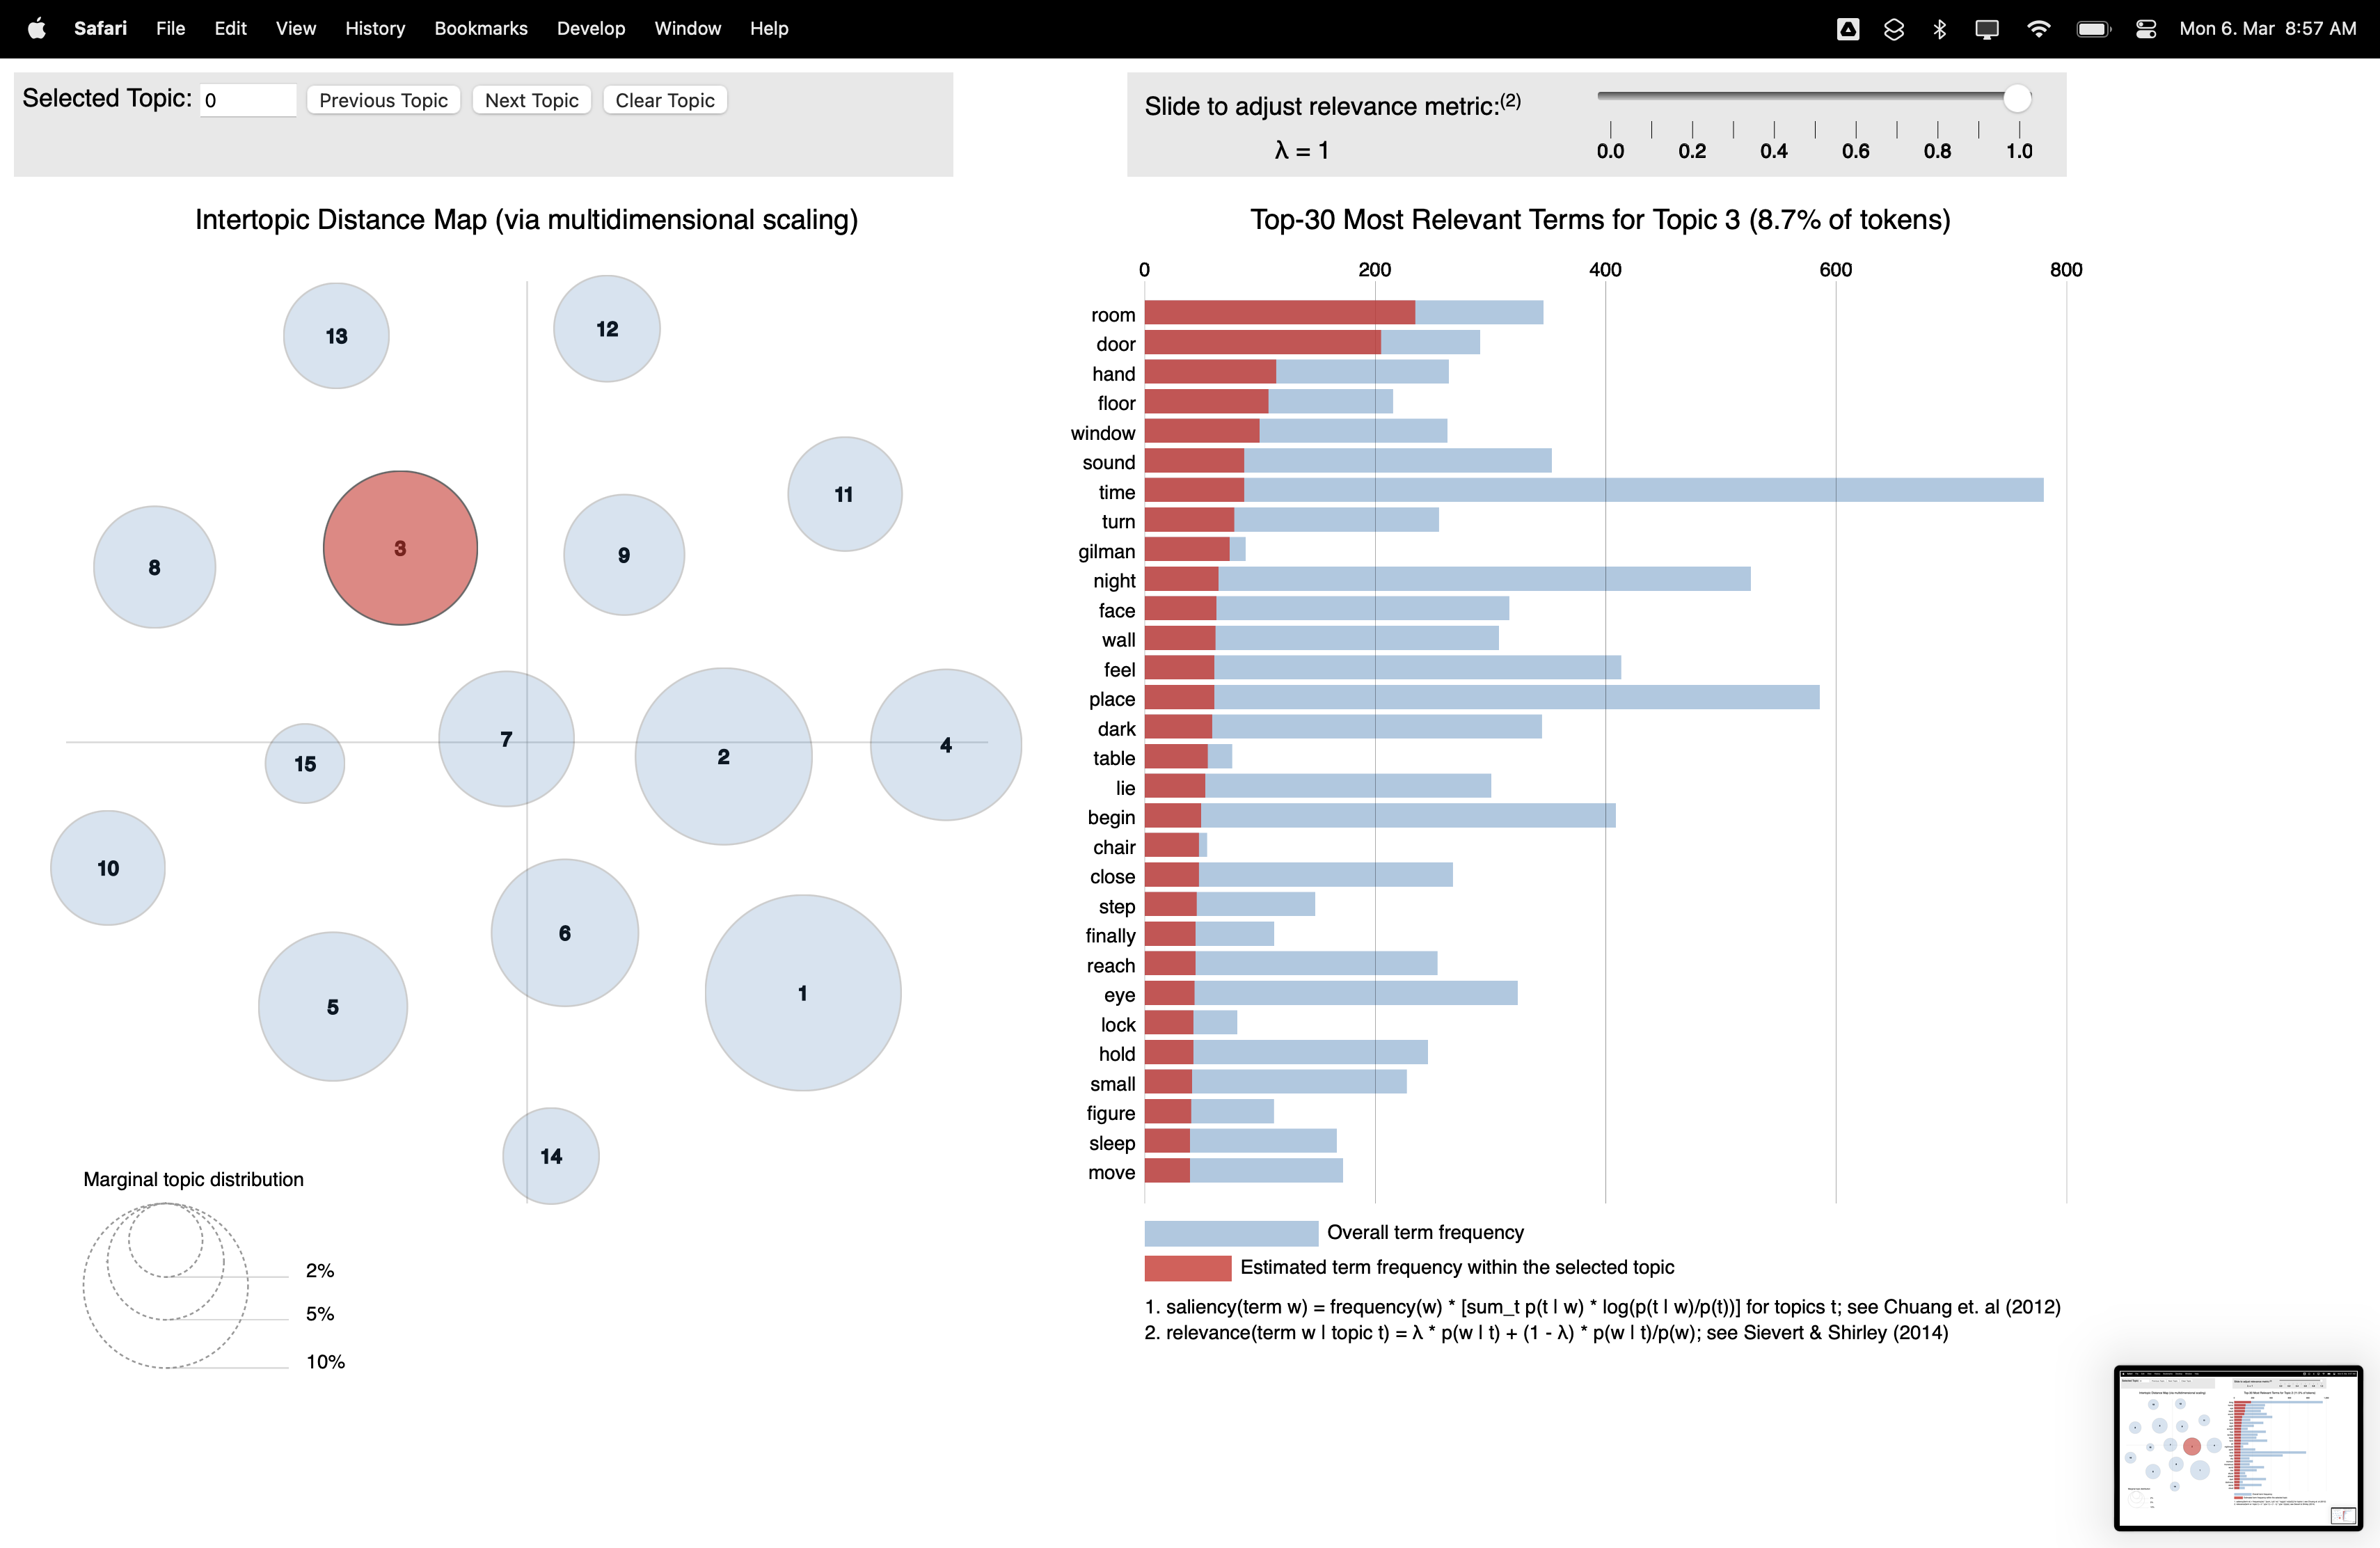
\includegraphics[width=1\textwidth]{/Users/ferriskleier/PECK/DigitalHumanities/Lovecraft_TopicModel/results/LDAvis_lambda-1/ldavis_L-1_03.png}
    \caption{LDAvis results, selected topic 3, $\lambda=1.0$}
    \label{fig:mesh3}
\end{figure}

\begin{figure}[p]
    \centering
    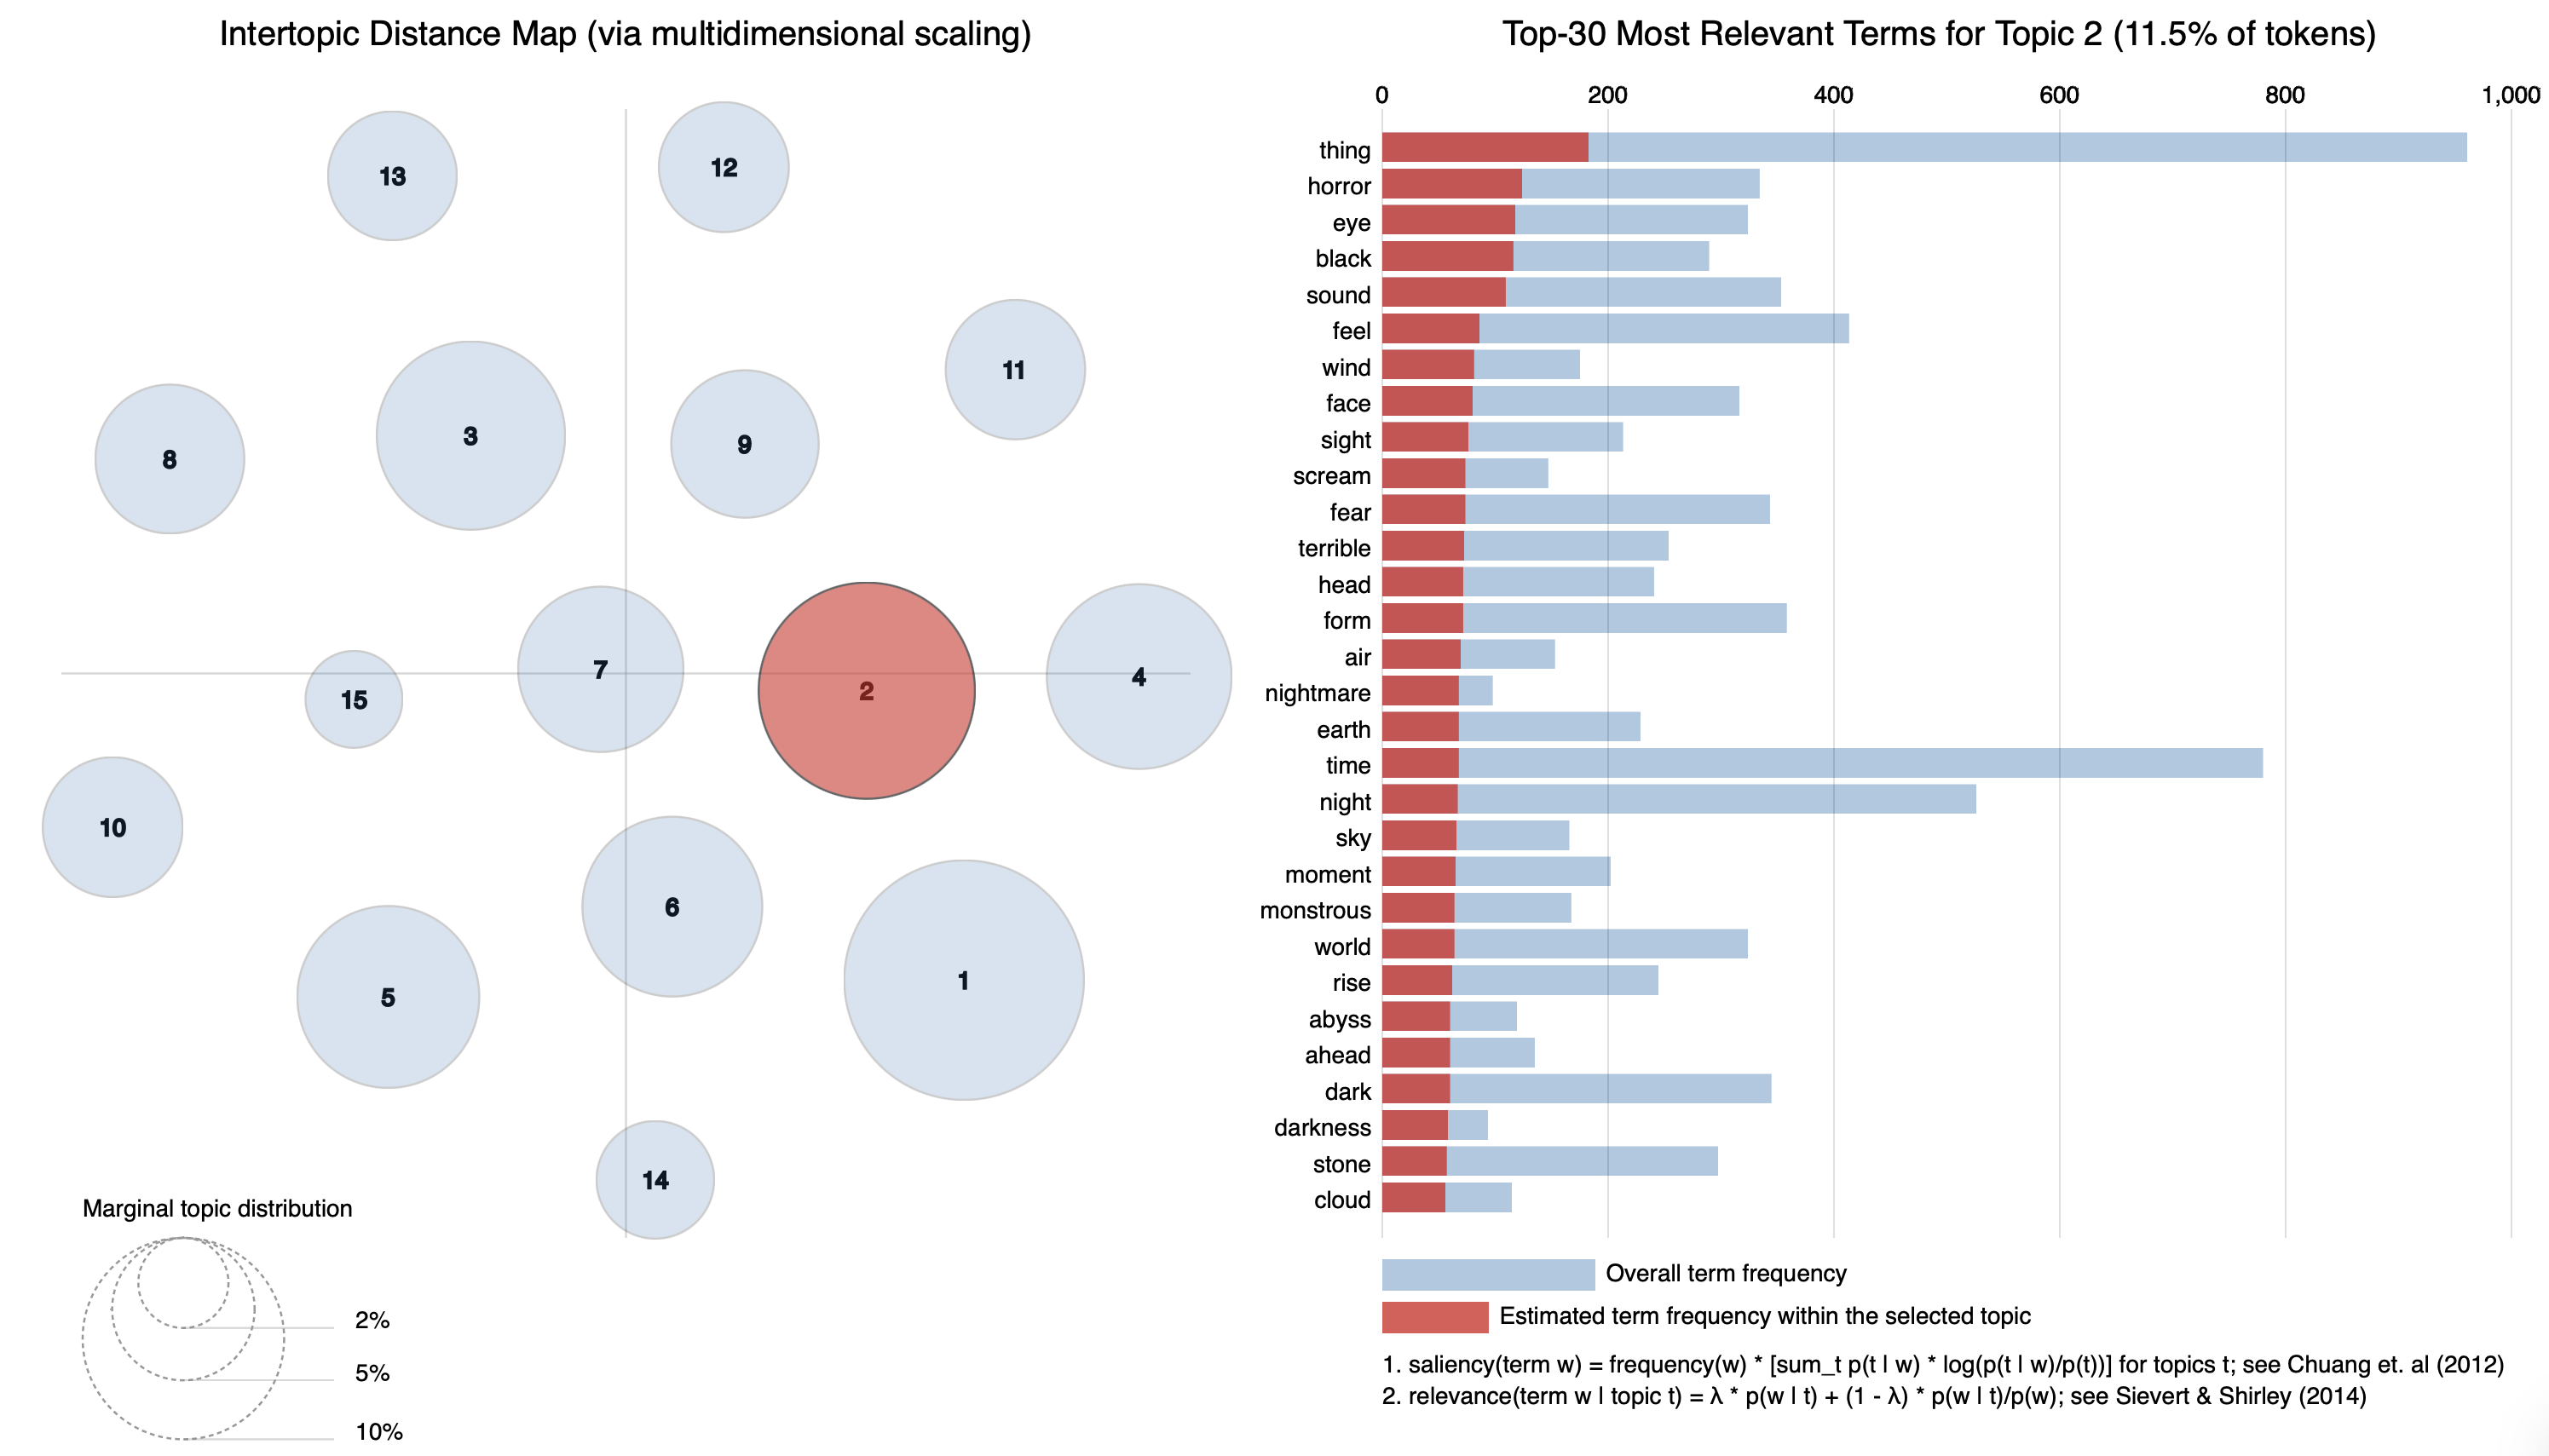
\includegraphics[width=1\textwidth]{/Users/ferriskleier/PECK/DigitalHumanities/Lovecraft_TopicModel/results/LDAvis_lambda-1/ldavis_L-1_02.png}
    \caption{LDAvis results, selected topic 2, $\lambda=1.0$}
    \label{fig:mesh4}
\end{figure}

We also used the R library LDAvis to find correlations between these topics or terms that are heavily 
linked to them. Figure 2 shows the resulting web interface from the topic model we got. The frequency 
of terms is shown on the right side of the plot. The plot represents each topic according to its 
importance within the topic model. The larger the circle, the more important this topic is. The use of 
LDAvis comes in convenient when we click on one of these circles representing a topic. As you can see 
in figure 3, the terms in relation to topic 3 are represented on the right-hand side. For this example, 
we can see that the words room and door are strongly connected to the other terms in that topic. There 
is also a slider to adjust the value for Lambda, which gives less relevant but more frequent terms in 
connection with the topic if Lambda is lower.\\

In context to Lovecraft’s life and insights from the first plot in figure 1, we can focus on some 
topics around already mentioned events. The first is the beginning of the dream cycle in 1920, covered 
by topic 3. As expected we can find a lot of terms relating to the topic of the dream cycle like room, 
sound, night, dark, and time. Stories around the dream cycle are typically not dreams but protagonists 
exploring otherworldly places. That way works 30 and 31 (‘The Quest of Iranon’ and ‘Ex Oblivione’) can 
be described using these relevant terms. One common share across these relevant terms for topic 3 is a 
vague description of the places, feelings, and situations it takes place in, matching Lovecraft’s 
writing of most of the works from the dream cycle according to dreams he had himself.\\



As seen in figure 4, Topic 2, which is associated with the time around his mother’s death, is 
connected to matching terms like horror, fear, terrible, or nightmare. This undermines our expectation 
that topic 2, though also present in earlier works, becomes more present because of his mother’s death 
and yields a stable share for some time.\\

\begin{figure}[p]
    \centering
    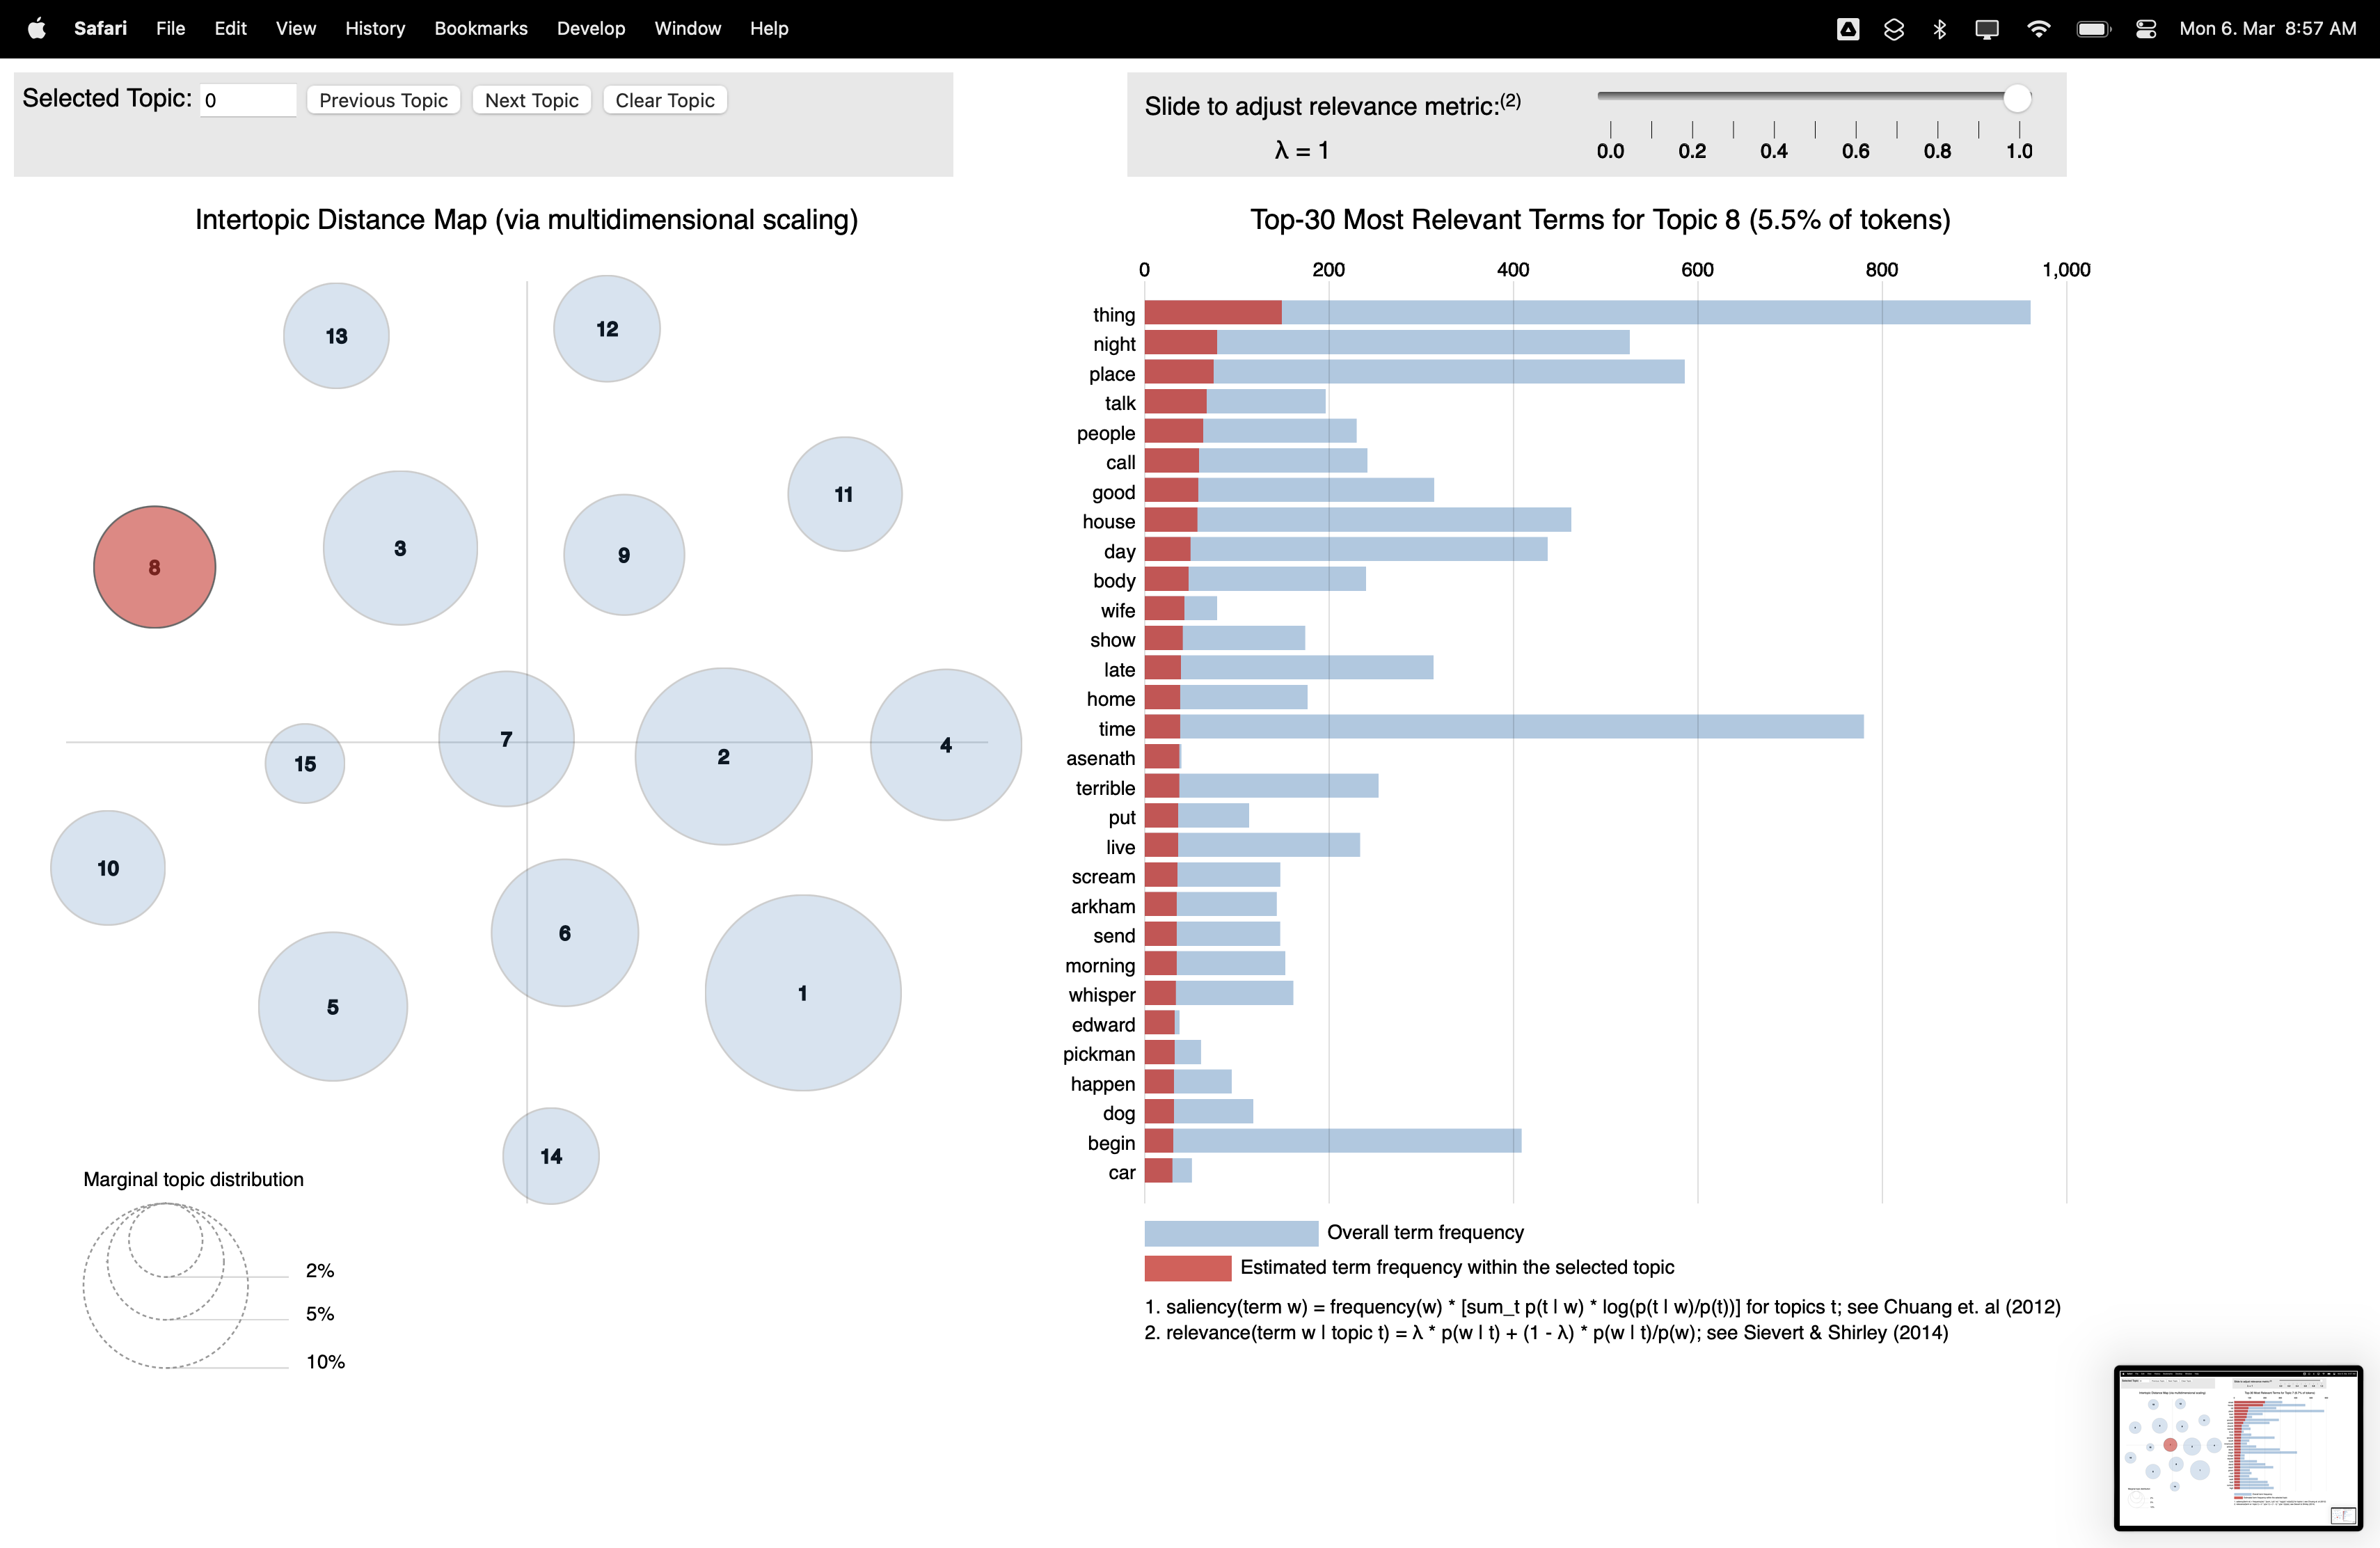
\includegraphics[width=0.49\textwidth]{/Users/ferriskleier/PECK/DigitalHumanities/Lovecraft_TopicModel/Project/images/ldavis_L-1_08.png}
    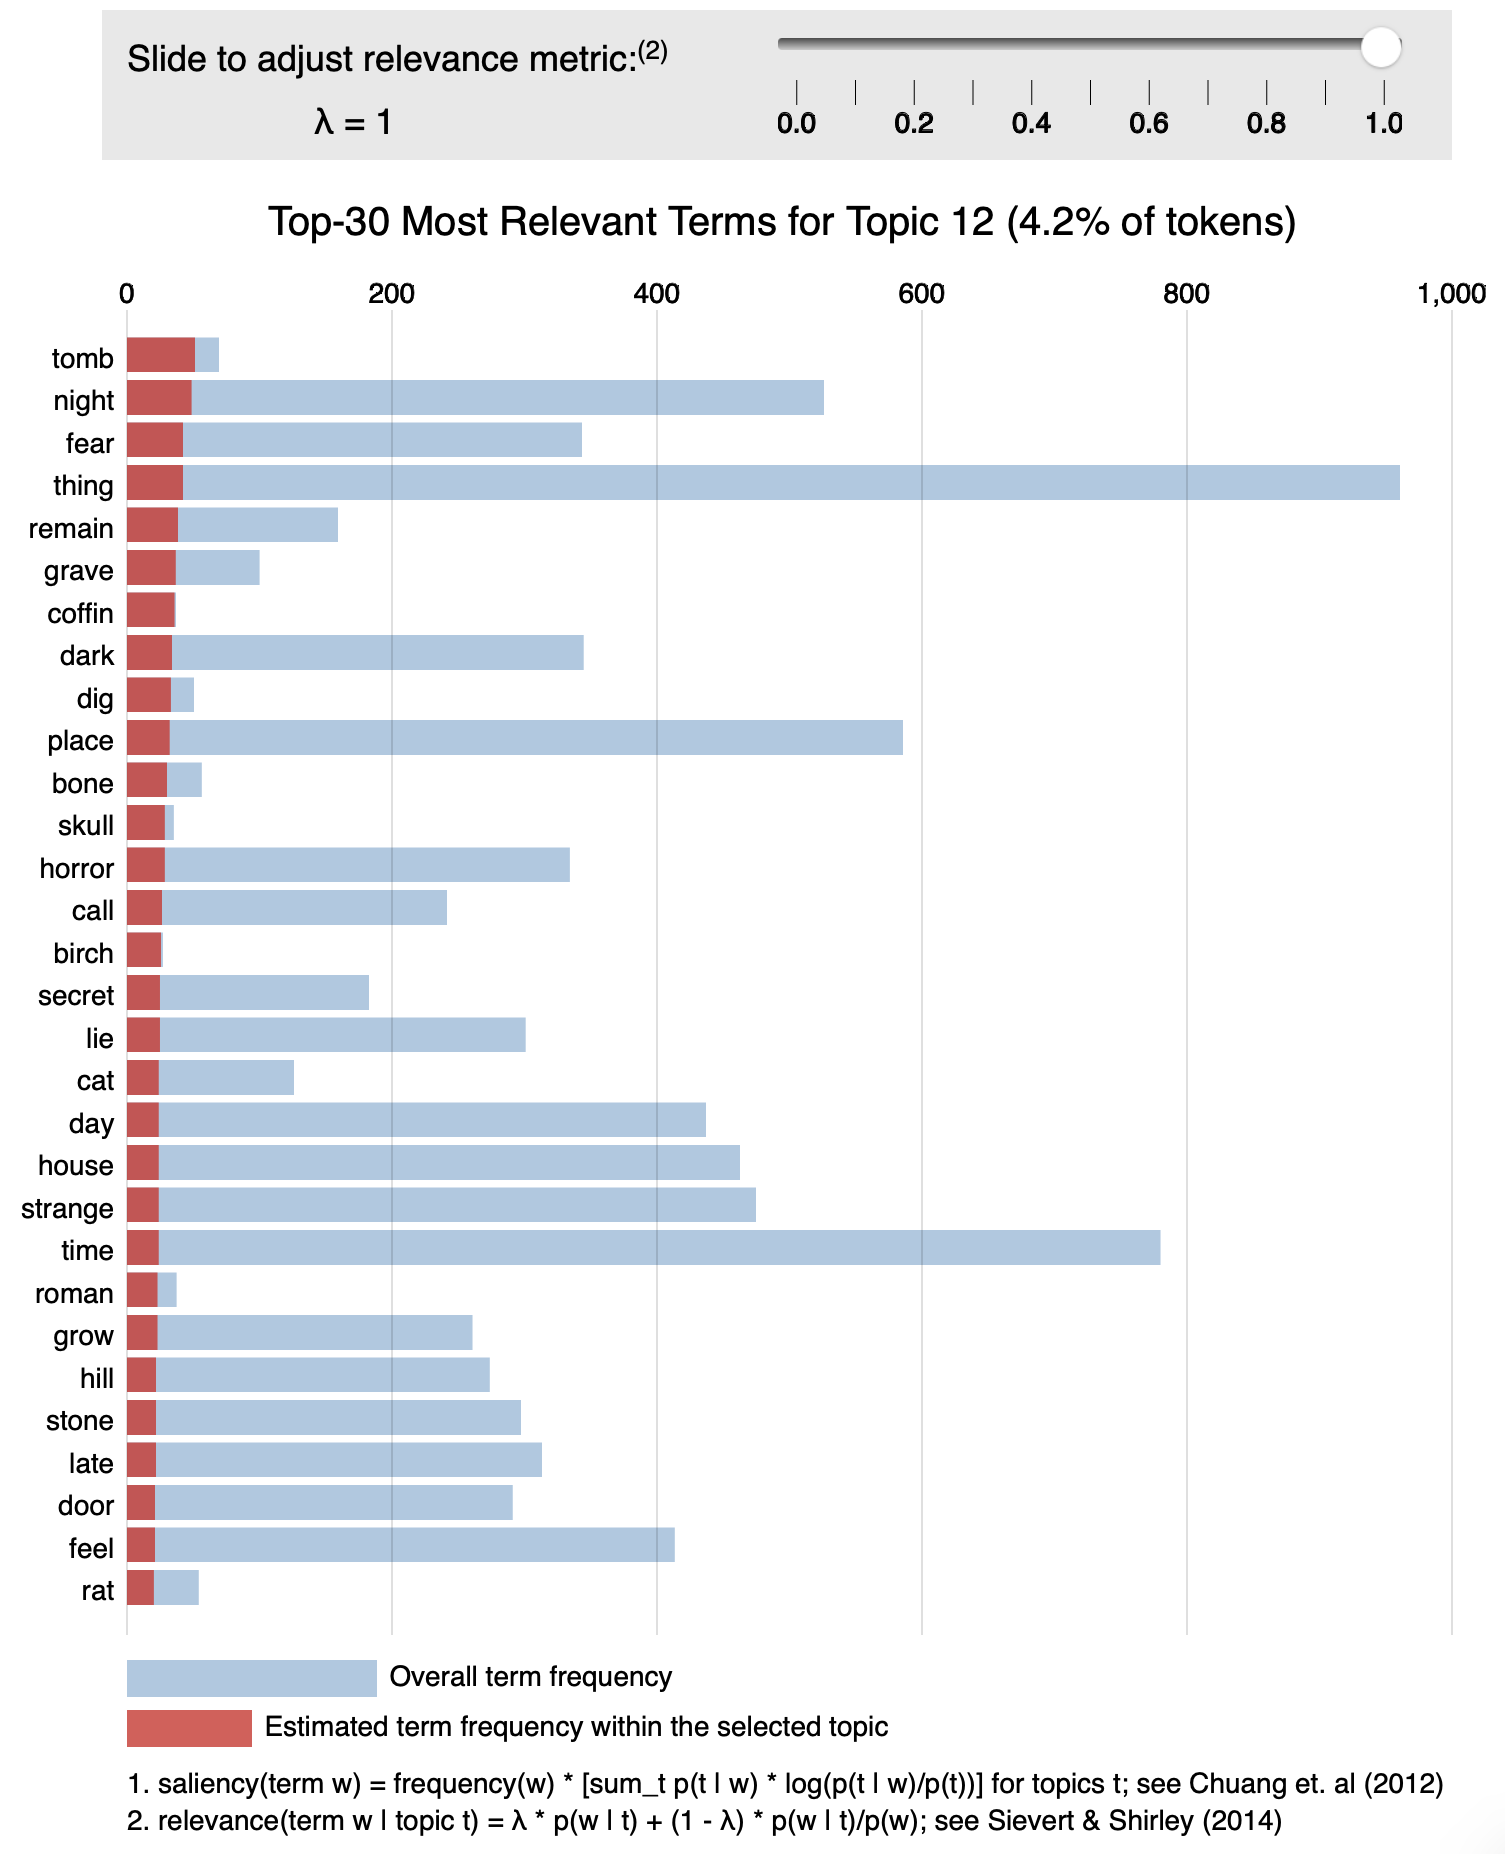
\includegraphics[width=0.49\textwidth]{/Users/ferriskleier/PECK/DigitalHumanities/Lovecraft_TopicModel/Project/images/ldavis_L-1_12.png}
    \caption{LDAvis results, selected topic 8 and 12, $\lambda=1.0$}
    \label{fig:mesh5}
\end{figure}

\begin{figure}[p]
    \centering
    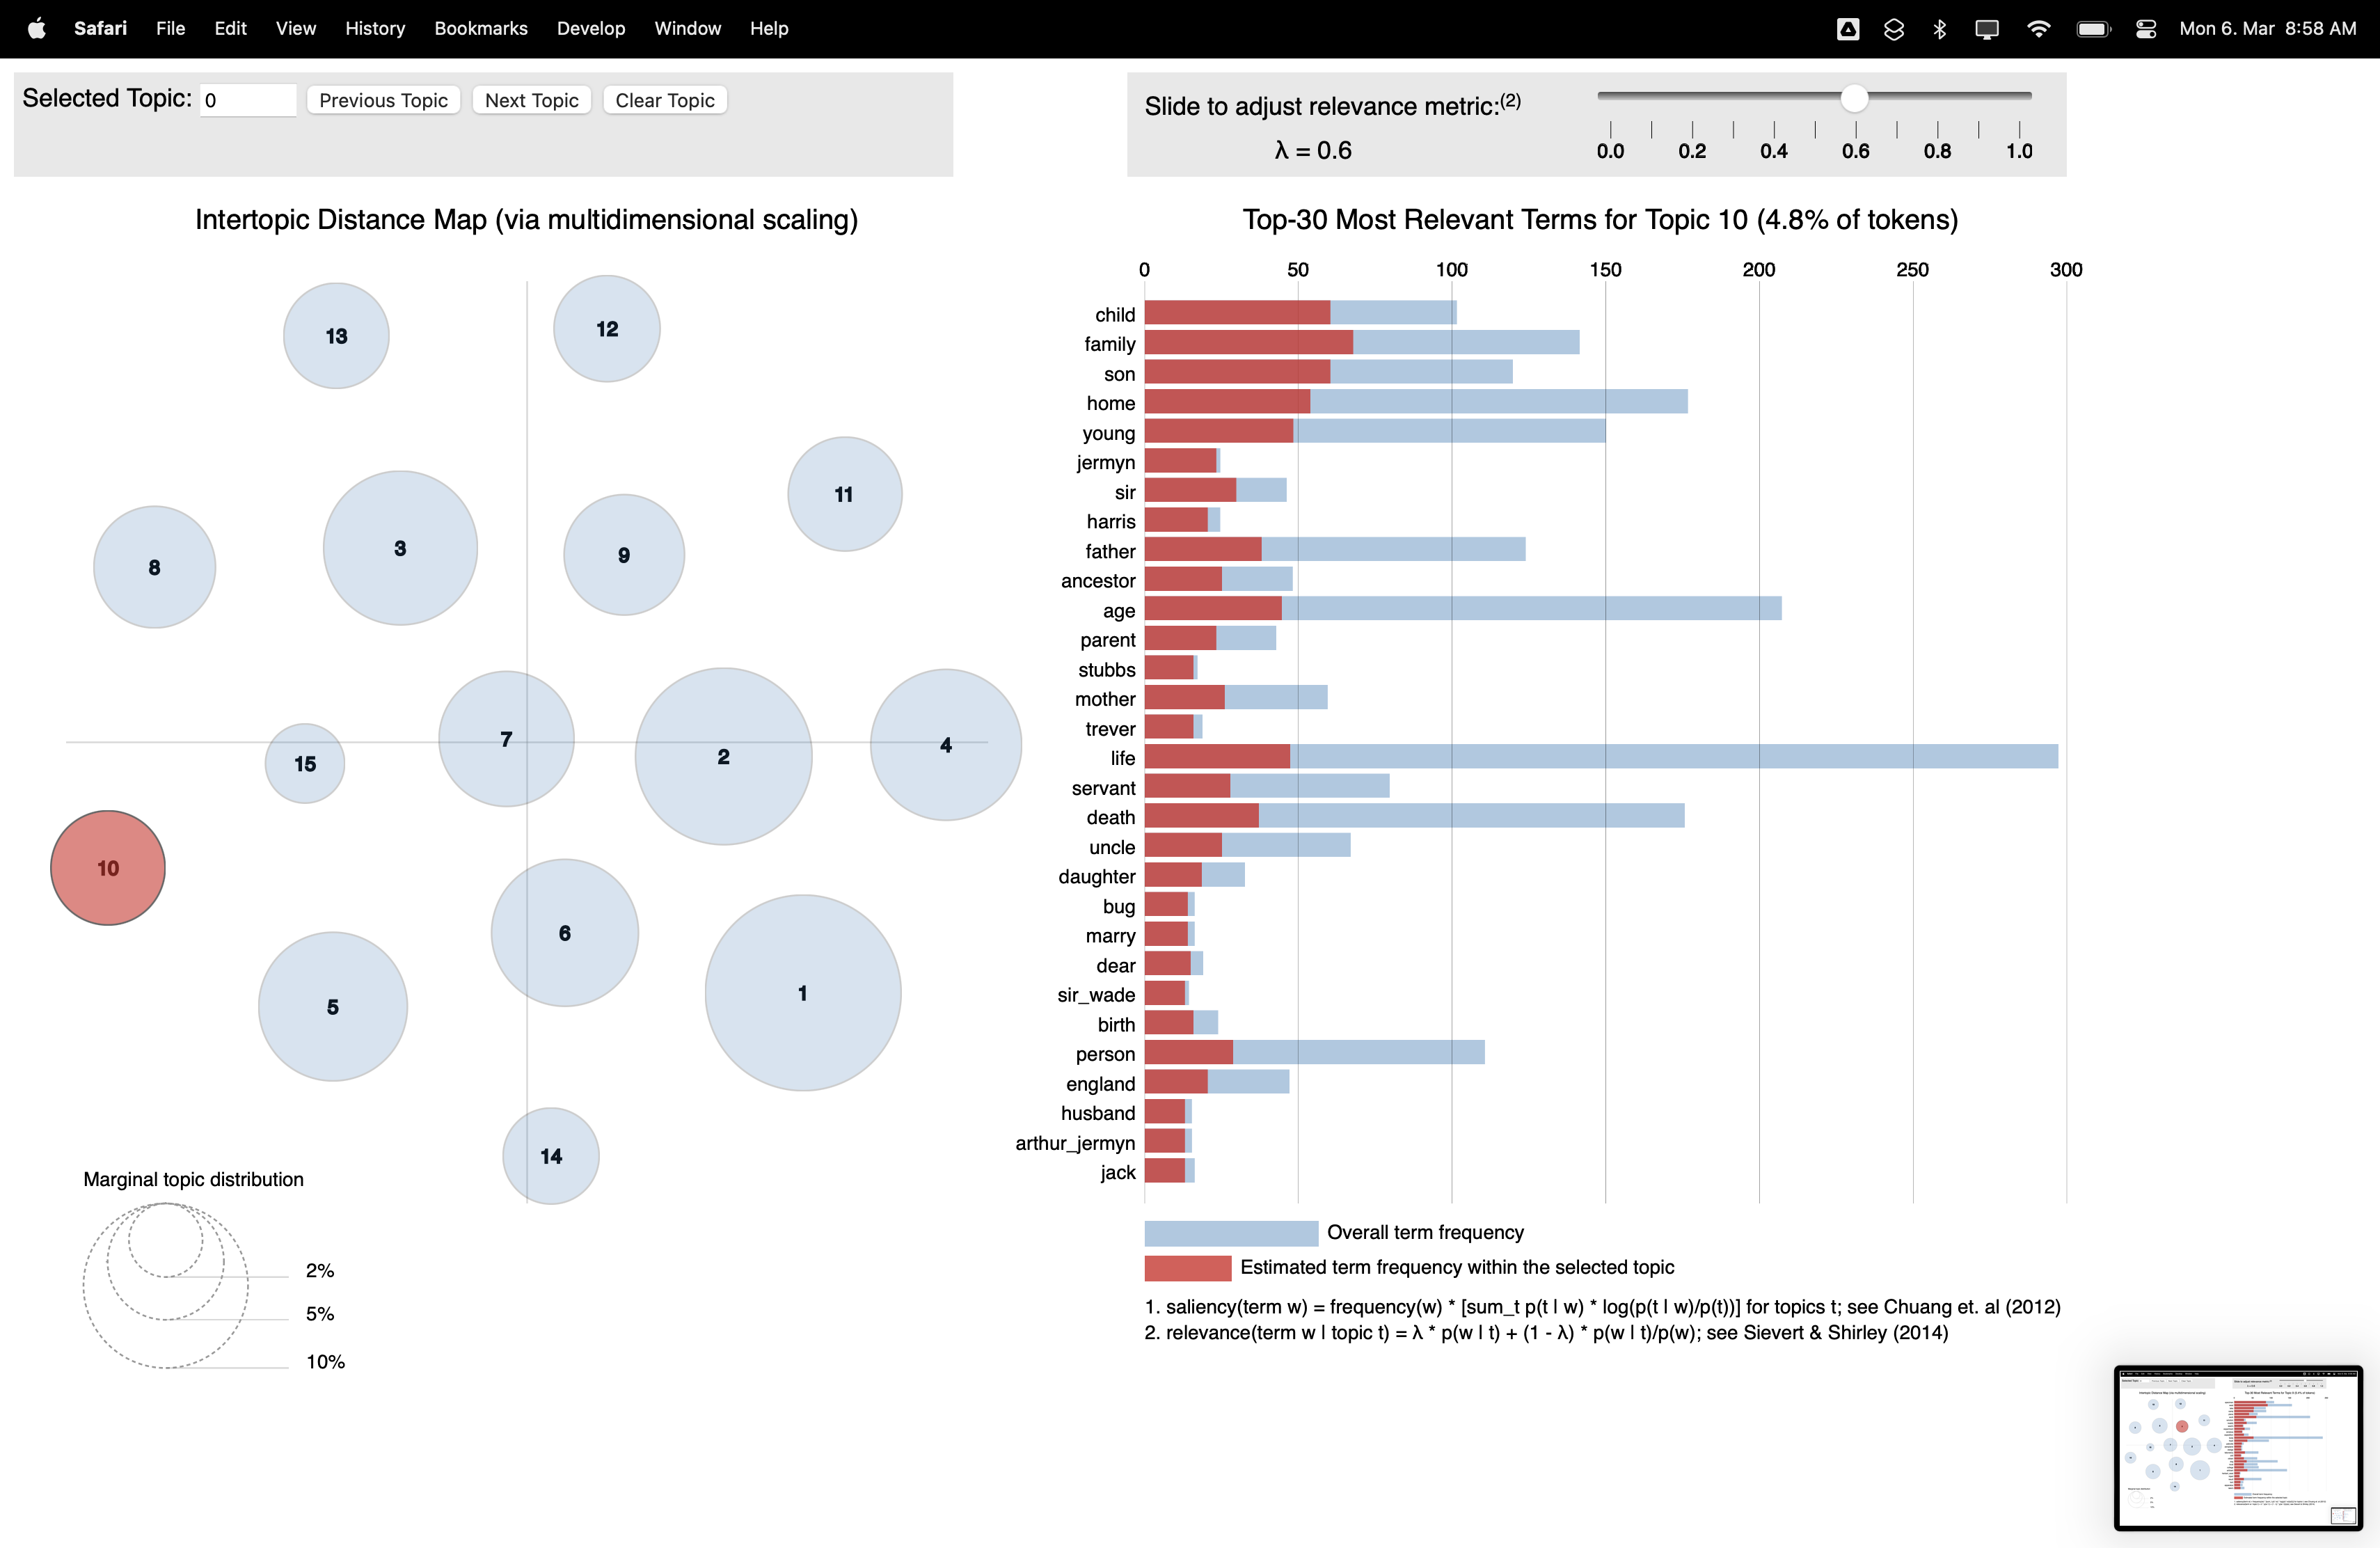
\includegraphics[width=1\textwidth]{/Users/ferriskleier/PECK/DigitalHumanities/Lovecraft_TopicModel/results/LDAvis_lambda-06/10.png}
    \caption{LDAvis results, selected topic 10, $\lambda=0.6$}
    \label{fig:mesh6}
\end{figure}

\begin{figure}[ht]
    \centering
    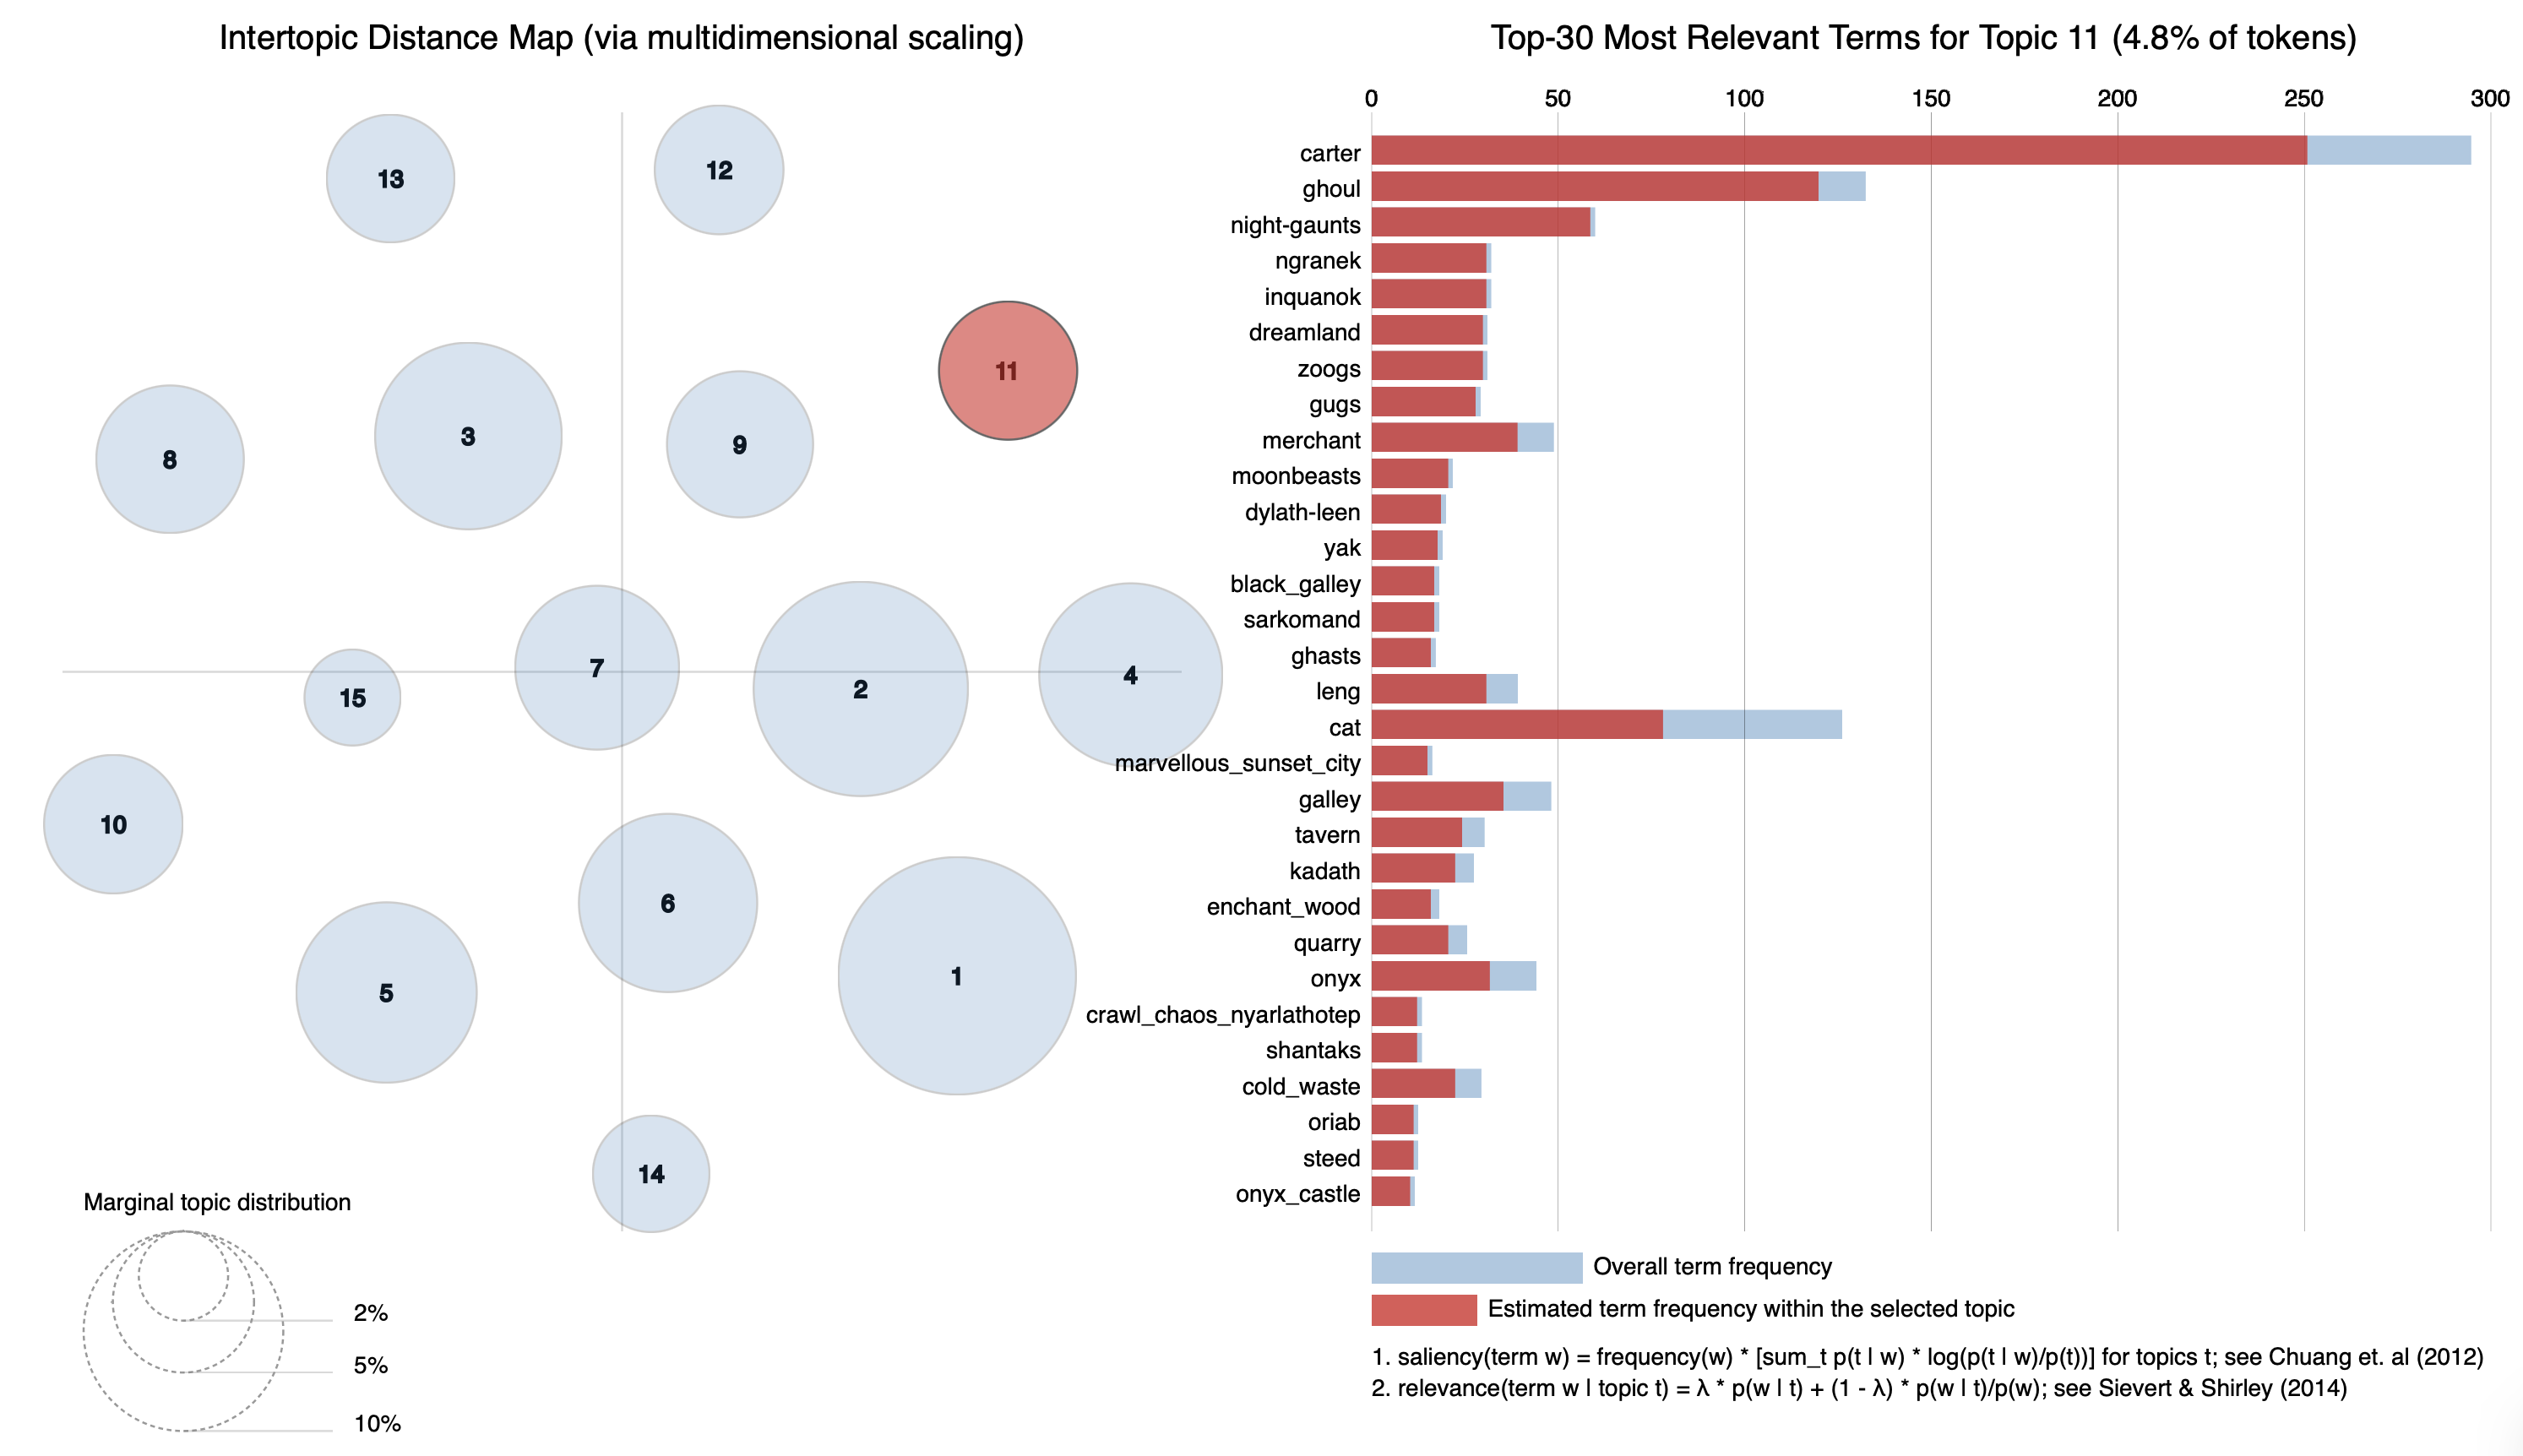
\includegraphics[width=1\textwidth]{/Users/ferriskleier/PECK/DigitalHumanities/Lovecraft_TopicModel/results/LDAvis_lambda-02/11.png}
    \caption{LDAvis results, selected topic 11, $\lambda=0.2$}
    \label{fig:mesh7}
\end{figure}

In figures 5 we can see the relevant terms for topics 8 and 12, which match closest to his stay 
in Brooklyn, cover place, people, wife, fear, and home. That is the most interesting insight because 
as we have seen in figure 1 one can find patterns in the time frames when he moved to Brooklyn and 
back to Providence. It is known that Lovecraft missed his home in Providence and ‘The Horror at 
Red Hook’ (written 1925) is a good indicator of his coping with the situation. As Lovecraft 
described the inspiration for that work himself in a letter to Clark Ashton Smith:

\begin{displayquote}
    \textit{The idea that black magic exists in secret today, or that hellish antique rites still exist in obscurity, is one that I have used and shall use again. When you see my new tale ‘The Horror at Red Hook’, you will see what use I make of the idea in connexion with the gangs of young loafers and herds of evil-looking foreigners that one sees everywhere in New York.}
\end{displayquote}

The last thing we want to cover is the fact that topic 10, which is present in most of his works 
but more frequent in his youth and later works as seen in figure 1, covers terms that do not directly 
indicate what lies behind them. As seen in figure 6, the terms of topic 10 have relevant terms 
including child, family, home, father, and other family-related terms. This may indicate phases 
where Lovecraft thought about his family during his youth or when his aunt was ill. A notable 
correlation can be found in topic 9, which covers these terms directly. As we can see in figure 
7, for topic 11, when Lambda is adjusted to less relevance but more frequency, relevant terms 
indicate a great share of the name Carter in this topic. Though topic 11 itself is not that special, 
the highest shares can be found in his early works and later works in figure 1. As mentioned earlier, 
Randolph Carter is a supposedly alter ego of Lovecraft. We think this an important part because it 
indicates when Lovecraft was working on this character and taking into account these phases of figure 
1 and the time he was in Providence, one can argue that he wrote on topics close to his alter ego 
during times of positivity and personal growth. These include the time around 1919/20 when he went 
to conventions and met other amateur authors as well as people he admired and the return to Providence. 
This becomes even more present with topic 15, which has the highest share in work 21, ‘The Cats of 
Ulthar’ (written 1920), and work 55, ‘The Dream Quest of Unknown Kadath (written 1927). Since topic 
15 contains Carter and cat as terms, we can link them to his personal experiences. Lovecraft loved 
cats and ‘The Cats of Ulthar’ is a clear representation of his admiration of these animals, 
supporting the idea of his alter ego even further.\\

Overall, though the terms do not directly represent any major events of his life, there are 
observable shifts in the themes of his writings around important events. One is the dream cycle, 
which stems from Lord Dunsany’s influence on Lovecraft. The big change in topics observable around 
work 33 in figure 1 clearly indicated his mother’s death. And even though his time in New York, 
which he despised, is only vaguely present in the topics 8 and 12, one can see the shift back to 
the topics around the dream cycle being present again after he moved back to providence (around 
work 50, in 1926). In the years before his divorce and after one can also see topic 7 having a 
slightly higher share, as well as a change in topics around his aunt's death in 1932 (from work 
66). A collection of screenshots of the LDAvis interface for Lambda values 0.2, 0.6, and 1.0 as 
well as the plot representing the topic model of all his works can be found in our repository in 
the folder results.

    \section{Conclusion}

In this project, we aimed to find correlations between Lovecraft’s personal life events and the main 
themes of his writings. For this purpose, we used the digital humanities, particularly topic modeling, 
to gather the main topics across Lovecraft’s works and their respective share for each work. We also 
used a web interface to find relevant terms for each topic, this added further depth to the insights 
we got.\\

The research question could be answered with good satisfaction since we clearly found patterns in 
the represented model that correlate to events of his life. Such include his mother’s death, the 
move to Brooklyn, his return to Providence, and divorce, as well as his aunt’s death. Though we 
expected some even more visible patterns, we found a good amount of links to these events when 
comparing the dates his works were written with the dates of the events. It’s also necessary to 
note that for some topics, the correlating event like his mother’s death or his divorce may have 
impacted some works even earlier. This is because the writing of a story is not completed in a 
short time and we took this into account when discussing his divorce’s influence, which may have 
been a topic for him earlier to the official divorce with problems in the relationship. We also 
got some key insights into one of the most important motifs of Lovecraft. Contrary to popularity, 
the most important works do not cover the ‘Cthulhu Mythos’, which Lovecraft is most known for today, 
but the ‘Dream Cycle’ and Lovecraft’s personal input like his supposed alter ego Randolph Carter, 
his love for cats, and the dreams that influenced his writings.\\

From the distribution of topics and their relevant terms, it’s also slightly observable when 
Lovecraft moved to Brooklyn and returned to Providence, marking a break in his dream cycle and 
a return to more cosmic horror and self-fulfillment when he was back in his hometown. The last 
few works cover a mix of topics with no clear patterns that could also be described by his shift 
towards ghostwriting and fictional stories becoming less frequent and richer in length. Social 
events of that time, like World War 1 or the great depression could not be clearly linked to and 
were therefore not covered.\\

It’s important to mention that this project is just the foundation of possible research on his 
life-work correlation using digital methods like LDA and machine learning. Future work regarding 
the digital humanities may not only include topic modeling on his fictional works but also his 
non-fiction and letters. It’s also interesting to bring up stylometry as a method here, where 
we could see shifts in his stylistic devices that may correlate to personal events of his as 
well. Overall, this project has shown the potential of topic modeling as a tool for literary 
analysis and its ability to uncover previously unknown patterns in a body of text. It contributes 
to the ongoing research of Lovecraft’s works in the digital age and offers notable insights and 
foundations for such future work.

    \newpage

\begin{thebibliography}{9}
\itemsep0em

\bibitem{wohleber}
Wohleber, C. (1995). \emph{The Man Who Can Scare Stephen King}. Retrieved Feb 17 2023, from \href{https://www.americanheritage.com/man-who-can-scare-stephen-king}{https://www.americanheritage.com/man-who-can-scare-stephen-king}

\bibitem{kirschenbaum}
Kirschenbaum, M. (2010). \emph{What Is Digital Humanities and What's It Doing in English Departments?}. Retrieved Feb 17 2023, from \href{https://dhdebates.gc.cuny.edu/read/untitled-88c11800-9446-469b-a3be-3fdb36bfbd1e/section/f5640d43-b8eb-4d49-bc4b-eb31a16f3d06}{https://dhdebates.gc.cuny.edu/read/untitled-88c11800-9446-469b-a3be-3fdb36bfbd1e/section/f5640d43-b8eb-4d49-bc4b-eb31a16f3d06}

\bibitem{nyhan}
Nyhan, J., \& Plotnikova, M. (Eds.). (2019). \emph{One origin of Digital Humanities}. Springer International Publishing.

\bibitem{romano}
Romano, A. (2020). \emph{Lovecraftian horror — and the racism at its core — explained}. Retrieved Feb 21 2023, from \href{https://www.vox.com/culture/21363945/hp-lovecraft-racism-examples-explained-what-is-lovecraftian-weird-fiction}{https://www.vox.com/culture/21363945/hp-lovecraft-racism-examples-explained-what-is-lovecraftian-weird-fiction}

\bibitem{lc}
H. P. Lovecraft bibliography (2023). In \emph{Wikipedia}. Retrieved Feb 21 2023, from \href{https://en.wikipedia.org/w/index.php?title=H._P._Lovecraft_bibliography&oldid=1135325435}{https://en.wikipedia.org/w/index.php?title=H.\_P.\_Lovecraft\_bibliography\&oldid=1135325435}

\bibitem{joshi}
Joshi, S. T., \& Schultz, D. E. (2001). \emph{An H. P. lovecraft encyclopedia}. Greenwood Press. 

\bibitem{wiki}
Author:Howard Phillips Lovecraft (2023). In \emph{Wikisource} . Retrieved Mar 7 2023, from \href{https://en.wikisource.org/w/index.php?title=Author:Howard_Phillips_Lovecraft&oldid=12959276}{https://en.wikisource.org/w/index.php?title=Author:Howard\_Phillips\_Lovecraft\&oldid=12959276}

\bibitem{blei}
Blei, D. (2012). \emph{Topic Modeling and Digital Humanities}. Retrieved Mar 01 2023, from \href{https://journalofdigitalhumanities.org/2-1/topic-modeling-and-digital-humanities-by-david-m-blei/}{https://journalofdigitalhumanities.org/2-1/topic-modeling-and-digital-humanities-by-david-m-blei/}

\bibitem{gusta}
Gustafson, K. (2005). \emph{Beyond the mountain of madness : a look at the shared themes of Edgar Allan Poe and H.P. Lovecraft (Dissertation)}. Retrieved from \href{http://urn.kb.se/resolve?urn=urn:nbn:se:ltu:diva-43672}{http://urn.kb.se/resolve?urn=urn:nbn:se:ltu:diva-43672}

\bibitem{wiki2}
Supernatural Horror in Literature (2023). In \emph{Wikisource}. Retrieved Mar 07 2023, from \href{https://en.wikisource.org/w/index.php?title=Supernatural_Horror_in_Literature&oldid=12891211}{https://en.wikisource.org/w/index.php?title=Supernatural\_Horror\_in\_Literature\&oldid=12891211}

\bibitem{church}
Church, M. A. (2013). \emph{The Lovecraft Look: An Examination of Lovecraftian Themes in Film}. Find at \href{https://digitalcommons.buffalostate.edu/english\_theses/11}{https://digitalcommons.buffalostate.edu/english\_theses/11}

\bibitem{smith}
Smith, P. (2011). \emph{Re-visioning Romantic-Era Gothicism: An Introduction to Key Works and Themes in the Study of H.P. Lovecraft}. Retrieved Mar 01 2023, from \href{https://doi.org/10.1111/j.1741-4113.2011.00838.x}{https://doi.org/10.1111/j.1741-4113.2011.00838.x}

\bibitem{holmes}
Holmes, F. (2022). \emph{Determining the Number of Topics to Retain using Tools from Factor Analysis}. Vol. 11, No. 1, 1-14. Find at \href{https://doi.org/10.47260/jsem/1111}{https://doi.org/10.47260/jsem/1111}

\bibitem{schultz}
Schultz, D. E., \& Joshi, S. T. (Eds.) (2011). \emph{An epicure in the Terrible: A centennial anthology of essays in honor of H.P. Lovecraft}. New York, NY. Hippocampus Press. 

\bibitem{joshi2}
Joshi, S. T. (1996). \emph{A Subtler Magick: The Writings and Philosophy of H.P. Lovecraft (Third ed.)}. Berkeley Heights, NJ. Wildside Press. page 79

\bibitem{carter}
Carter, L. (1996). \emph{Lovecraft: A look behind the "Cthulhu mythos"}. San Bernardino, CA. Borgo Press. 

\bibitem{letter}
Lovecraft, H.P. (1968). \emph{H. P. Lovecraft, Selected Letters vol. 2}. United States. Arkham House, p. 27

\end{thebibliography}

\end{document}
